% ============================================================
%  BiLSTM-GMM — Full Conference / Journal Paper
%  Compile on Overleaf:  pdflatex -> bibtex -> pdflatex x2
%  Place all PNG figures in a sub-folder named  figures/
%  (copy sda_results/fig01_data_distribution.png -> figures/, etc.)
% ============================================================

\documentclass[12pt,a4paper]{article}

% ---------- PACKAGES ----------
\usepackage[top=2.5cm, bottom=2.5cm, left=3.0cm, right=3.0cm]{geometry}
\usepackage{amsmath,amssymb,amsfonts,mathtools}
\usepackage{bm}
\usepackage{graphicx}
\usepackage{booktabs}
\usepackage{multirow}
\usepackage{array}
\usepackage{tabularx}
\usepackage{longtable}
\usepackage[numbers,sort&compress]{natbib}
\usepackage[colorlinks=true,linkcolor=blue!70!black,citecolor=blue!70!black,
            urlcolor=blue!70!black]{hyperref}
\usepackage{xcolor}
\usepackage{caption}
\usepackage{subcaption}
\usepackage{float}
\usepackage{microtype}
\usepackage{setspace}
\usepackage[T1]{fontenc}
\usepackage{lmodern}
\usepackage{parskip}
\usepackage{enumitem}
\usepackage{algorithm}
\usepackage{algpseudocode}
\usepackage{titlesec}
\usepackage{fancyhdr}
\usepackage{lastpage}

% ---------- FORMATTING ----------
\onehalfspacing
\setlength{\parindent}{1.5em}
\setlength{\parskip}{4pt}

\titleformat{\section}{\large\bfseries\sffamily}{\thesection.}{0.7em}{}[\titlerule]
\titleformat{\subsection}{\normalsize\bfseries\sffamily}{\thesubsection}{0.7em}{}
\titleformat{\subsubsection}{\normalsize\itshape}{\thesubsubsection}{0.7em}{}
\titlespacing{\section}{0pt}{14pt}{6pt}
\titlespacing{\subsection}{0pt}{10pt}{4pt}

\pagestyle{fancy}
\fancyhf{}
\rhead{\small BiLSTM-GMM for Seismic Ground Motion Prediction}
\lhead{\small}
\cfoot{\small Page \thepage\ of \pageref{LastPage}}
\renewcommand{\headrulewidth}{0.4pt}

% doi macro — renders as a clickable hyperlink (no extra package required)
\newcommand{\doi}[1]{\href{https://doi.org/#1}{\texttt{doi:\allowbreak#1}}}

\captionsetup{font=small,labelfont=bf,skip=4pt}
\graphicspath{{figures/}}

% ---------- DOCUMENT ----------
\begin{document}

% ===================================================================
%  TITLE PAGE
% ===================================================================
\begin{titlepage}
\centering
\vspace*{1.5cm}

{\LARGE\bfseries\sffamily
Spectral-Sequence Learning for Seismic Ground Motion\\ Prediction:
A Bidirectional LSTM Ground Motion Model\\[0.4em]
for Simultaneous Multi-Output Intensity Measure Estimation
\par}

\vspace{1.2cm}
{\large Mohamed Zayaan\par}
\vspace{0.3cm}
{\normalsize
Department of Civil \& Environmental Engineering\\
Seismic Data Analytics Research Group\\[0.2em]
\textit{Submitted April 2026}
\par}

\vspace{1.5cm}
\noindent\rule{\textwidth}{1pt}

\begin{abstract}
\noindent
Ground motion models (GMMs) predict seismic intensity measures (IMs) as
probabilistic functions of earthquake source, propagation path, and site
parameters, forming the computational backbone of probabilistic seismic
hazard analysis (PSHA).
Existing machine learning GMMs treat each spectral period as an
\emph{independent} regression target, discarding the strong physical
correlation that links adjacent spectral ordinates and ignoring the ordered
structure of the pseudo-spectral acceleration (PSA) response spectrum.
We present the \textbf{Seismic Bidirectional LSTM Ground Motion Model
(BiLSTM-GMM)}, which reformulates multi-output spectral prediction as a
\emph{sequence-to-sequence} learning problem in which period ordering
carries explicit physical meaning.
The model employs a dual-branch architecture: (i)~a feature encoder MLP with
residual skip connections maps eight physics-informed input features to a
shared context vector, and (ii)~a continuous period-embedding MLP maps
log-scaled pseudo-periods to a 64-dimensional spectral embedding.
The fused representations are processed by a two-layer bidirectional LSTM
that captures spectral correlation simultaneously in the short- and long-period
directions.
A physics-informed spectral-smoothness regulariser further encourages
physically plausible spectral shapes.
Trained and evaluated on 13{,}495 quality-controlled NGA-Subduction records
spanning $M_w$ 4.9--9.1, $R_{jb}$ 0--800~km, and $V_{s30}$
100--2\,000~m/s, the model simultaneously predicts PGA, 28 PSA ordinates at
periods 0.01--10~s, and PGV (30 IMs total) with a held-out test
coefficient of determination $R^2 = 0.925$ and root-mean-square error
(RMSE) $= 0.673$ natural-log units.
Per-IM Pearson correlation coefficients range from $r = 0.916$ (PSA at 2~s)
to $r = 0.956$ (PSA at 10~s), competitive with state-of-the-art empirical and
neural-network GMMs.
Sensitivity analysis confirms physically expected scaling with magnitude,
distance, site condition, and rupture depth, while SHAP-based attribution
identifies log-scaled Joyner-Boore distance and $M_w \times \ln R_{jb}$ as
the dominant predictors.
\end{abstract}
\noindent\rule{\textwidth}{1pt}

\vspace{0.6cm}
\noindent
\textbf{Keywords:}
seismic ground motion model;\enspace
bidirectional LSTM;\enspace
pseudo-spectral acceleration;\enspace
NGA-Subduction;\enspace
probabilistic seismic hazard;\enspace
machine learning GMM;\enspace
multi-output regression;\enspace
spectral correlation

\end{titlepage}

% ===================================================================
%  1. INTRODUCTION
% ===================================================================
\section{Introduction}
\label{sec:intro}

Probabilistic seismic hazard analysis (PSHA) relies critically on the accuracy
of ground motion models (GMMs), also called ground motion prediction equations
(GMPEs), which estimate the probability distribution of seismic intensity
measures (IMs) conditional on earthquake source and site parameters
\citep{Cornell1968,McGuire2004}.
The pseudo-spectral acceleration PSA$(T)$---the maximum response of a
single-degree-of-freedom oscillator at natural period $T$---is the most
widely used IM in structural engineering because it directly characterises the
forcing experienced by buildings.
Accurate spectral predictions across the full period range (0.01--10~s) are
therefore essential for reliable seismic risk assessments.

Subduction-zone earthquakes represent some of the most energetic seismic events
on Earth: megathrust interface events ($M_w > 8$) produce prolonged ground
shaking with rich long-period energy that differs fundamentally from crustal
ground motion \citep{Zhao2006,Abrahamson2016}.
The NGA-Subduction research programme \citep{Bozorgnia2014} has assembled the
largest curated flatfile of subduction recordings, enabling the development of
new empirical GMMs specifically calibrated to interface and intraslab events in
the Pacific Rim and other subduction environments.
Despite this progress, published empirical GMMs for subduction zones---such as
the BC~Hydro model \citep{Abrahamson2016} and those of \citet{Zhao2006} and
\citet{Atkinson2003}---are based on prescribed functional forms that may not
capture the full complexity of ground-motion scaling.

The application of machine learning (ML) to GMM development has grown rapidly
over the past decade.
Neural-network GMPEs \citep{Derras2014,Derras2016,Sahakian2018,
Khosravikia2021,Kuehn2015} demonstrate that flexible, data-driven models can
achieve lower residual variance than parametric GMMs while preserving physical
interpretability through careful feature engineering.
However, a fundamental limitation shared by virtually all existing ML GMMs is
that each spectral period is predicted \emph{independently}: the model at
period $T$ has no access to its predictions at neighbouring periods $T'$,
even though physical wave-propagation theory guarantees strong spectral
correlation.
As a result, independently predicted spectra can exhibit unphysical kinks,
crossing, or non-monotonic behaviour that must be post-processed.

Recurrent neural networks (RNNs)---and in particular long short-term memory
(LSTM) networks \citep{Hochreiter1997}---excel at sequential data by maintaining
a hidden state that propagates information across time steps.
Bidirectional LSTMs (BiLSTMs) \citep{Schuster1997} process sequences in both
directions and have achieved state-of-the-art performance on structured
prediction tasks in speech \citep{Graves2013}, natural language processing, and
biomedical signal processing.
Their direct application to the spectral prediction problem---treating period
index as a \emph{sequence axis}---is a natural and, to our knowledge, largely
unexplored direction in seismic GMM research.

This paper makes the following contributions:
\begin{enumerate}[leftmargin=*,label=\textbf{C\arabic*.}]
  \item \textbf{Spectral-sequence formulation.}
        We reformulate multi-output spectral GMM as a sequence problem, placing
        the 30 output IMs (PGA, PSA at 28 periods, PGV) in pseudo-period order
        so that period index carries physical meaning for the recurrent model.
  \item \textbf{Dual-branch architecture.}
        We separate the encoding of site/source/path features (Feature Encoder)
        from the encoding of oscillator period (Period Embedding MLP), fusing
        them before the BiLSTM to give the sequence model both contextual and
        spectral information at every step.
  \item \textbf{Continuous period embedding.}
        A small MLP maps $\ln T$ to a 64-dimensional embedding without
        discretisation, enabling the model to generalise to arbitrary periods not
        seen during training.
  \item \textbf{Physics-informed spectral regularisation.}
        A second-order finite-difference smoothness penalty, applied in $\ln$-IM
        space, enforces spectral continuity and penalises unphysical oscillations.
  \item \textbf{Physics-consistent evaluation.}
        We demonstrate that the trained model reproduces qualitatively and
        quantitatively expected ground-motion scaling with all four primary
        predictors: magnitude, distance, site condition ($V_{s30}$), and rupture
        depth ($Z_{tor}$).
\end{enumerate}

The remainder of the paper is organised as follows.
Section~\ref{sec:relwork} reviews related work.
Section~\ref{sec:data} describes the dataset and feature engineering.
Section~\ref{sec:arch} presents the BiLSTM-GMM architecture.
Section~\ref{sec:training} describes the training procedure.
Section~\ref{sec:results} reports quantitative and visual results.
Section~\ref{sec:discussion} discusses physical plausibility, limitations, and
broader implications.
Section~\ref{sec:conclusion} concludes.

% ===================================================================
%  2. RELATED WORK
% ===================================================================
\section{Related Work}
\label{sec:relwork}

\subsection{Empirical Ground Motion Models}

Classical GMMs express IM as an analytical function of source, path, and site
parameters, with free coefficients fitted by mixed-effects regression
\citep{Abrahamson2016,Boore2014,Campbell2014,Chiou2014}.
Mixed-effects formulations explicitly separate total residuals into
between-event ($\delta B$), site-to-site ($\delta S2S$), and within-event
($\delta WS$) components \citep{Al-Atik2010}.
Parametric functional forms provide physical interpretability but constrain
the model class; deviations from the assumed form introduce bias, particularly
in data-sparse regions of the predictor space (e.g., near-fault, very long
periods, and deep subduction).

\subsection{Machine Learning GMMs}

\citet{Derras2014,Derras2016} demonstrated that shallow neural networks
can produce GMPEs with total sigma comparable to parametric models for European
crustal events, using careful cross-validation to prevent overfitting.
\citet{Kuehn2015} explored Bayesian and penalised regression formulations.
\citet{Sahakian2018} trained a multilayer perceptron (MLP) for shallow crustal
ground motions in California, showing improved residual behaviour compared to
NGA-West2 models in certain magnitude--distance ranges.
\citet{Khosravikia2021} developed artificial-intelligence-based GMPEs calibrated
to Texas recordings.

In all of the above, each target IM (or spectral period) is predicted by a
separate model or by a shared model that treats period as an additional scalar
input but does not model period-to-period correlations explicitly.
This results in each spectrum being assembled from independently drawn samples,
which may violate spectral smoothness in individual predictions.

\subsection{Sequence Models in Seismology}

Recurrent architectures have found limited but growing application in
seismology: for earthquake detection and classification \citep{Perol2018},
seismogram denoising, and P-wave phase picking.
To our knowledge, the use of a bidirectional LSTM to simultaneously predict the
complete spectral response---treating period as a sequence axis---has not been
proposed previously in the GMM literature.
The closest related idea is the work of \citet{Bayona2022}, who apply deep
learning within a PSHA framework but focus on intensity measure selection rather
than spectral prediction architecture.

\subsection{Multi-Output and Structured Prediction}

Multi-task learning \citep{Caruana1997} and structured prediction
\citep{Bakir2007} provide theoretical frameworks for the joint modelling of
correlated outputs.
In the spectral GMM context, \citet{Baker2008} studied spectral correlation
for ground motion selection; \citet{Jayaram2009} modelled cross-period
correlations in GMMs using copulas.
These statistical models, however, are applied post-hoc and do not influence
the GMM predictions themselves.
Our BiLSTM-GMM learns spectral correlations directly from data as part of the
prediction process.

% ===================================================================
%  3. DATASET AND FEATURE ENGINEERING
% ===================================================================
\section{Dataset and Feature Engineering}
\label{sec:data}

\subsection{NGA-Subduction Flatfile}

We use the NGA-Subduction strong-motion flatfile \citep{Bozorgnia2014}, which
aggregates quality-controlled recordings from subduction environments world-wide,
including Japan, Cascadia, Chile, and Mexico.
The complete flatfile contains records spanning moment magnitude
$M_w \approx 4.5$--9.1, Joyner-Boore distances $R_{jb}$ 0--1\,000~km, and
$V_{s30}$ values 100--2\,000~m/s, with both interface and intraslab events.

\subsection{Data Cleaning and Sentinel Handling}

After removing records with missing or non-physical sentinel values
($R_{jb} = -999$~km and $V_{s30} \le 0$~m/s, totalling approximately 70
records), and dropping any record for which at least one target IM is
non-positive or non-finite, a total of \textbf{13{,}495 records} were
retained for modelling.
Fault type (focal mechanism) and the finite-fault-model indicator were filled
with their respective modal values where missing.

\subsection{Target Intensity Measures}

The model predicts 30 IMs simultaneously (Table~\ref{tab:IMs}):
peak ground acceleration (PGA, in units of $g$), pseudo-spectral acceleration
PSA$(T)$ at 28 oscillator periods spanning 0.01--10~s, and peak ground
velocity (PGV, in cm/s).
All IMs are modelled in natural-log space; targets are
$y_k = \ln(\text{IM}_k)$.
PGA is assigned pseudo-period $T_0 = 0.005$~s and PGV pseudo-period
$T_{29} = 15$~s for the purpose of period embedding, preserving the ordered
structure of the spectral sequence.

\begin{table}[htbp]
\centering
\caption{The 30 target intensity measures (IMs) in period order.
PGA and PGV are assigned pseudo-periods for sequence encoding.}
\label{tab:IMs}
\footnotesize
\renewcommand{\arraystretch}{1.15}
\begin{tabular}{clll}
\toprule
Index & IM & Period (s) & Units \\
\midrule
0  & PGA & 0.005 (pseudo) & $g$ \\
1--10 & PSA & 0.01, 0.02, 0.03, 0.04, 0.05, 0.06, 0.07, 0.08, 0.09, 0.10 & $g$ \\
11--19 & PSA & 0.20, 0.30, 0.40, 0.50, 0.60, 0.70, 0.80, 0.90, 1.00 & $g$ \\
20--28 & PSA & 2.0, 3.0, 4.0, 5.0, 6.0, 7.0, 8.0, 9.0, 10.0 & $g$ \\
29 & PGV & 15.0 (pseudo) & cm/s \\
\bottomrule
\end{tabular}
\end{table}

\subsection{Input Feature Engineering}
\label{sec:features}

Eight physics-motivated input features are used (Table~\ref{tab:features}).
Raw distance $R_{jb}$ is log-transformed to $\ln R_{jb}$ after flooring at
0.1~km to avoid $-\infty$ for on-fault ($R_{jb}=0$) records.
$V_{s30}$ is log-transformed to $\ln V_{s30}$.
Two interaction features, $M_w^2$ (quadratic magnitude scaling) and
$M_w \cdot \ln R_{jb}$ (magnitude-attenuation interaction), capture non-linear
source-path coupling consistent with standard GMM functional forms
\citep{Boore2014,Abrahamson2016}.

\begin{table}[htbp]
\centering
\caption{Input feature vector $\mathbf{x} \in \mathbb{R}^8$.}
\label{tab:features}
\footnotesize
\renewcommand{\arraystretch}{1.15}
\begin{tabular}{cll}
\toprule
Index & Feature & Physical meaning \\
\midrule
0 & $M_w$ & Moment magnitude \\
1 & $Z_{tor}$ (km) & Depth to top of rupture \\
2 & FFM & Finite-fault model flag (binary) \\
3 & $R_{jb}$ (km) & Joyner-Boore distance \\
4 & $\ln V_{s30}$ & Log site condition \\
5 & $\ln R_{jb}$ & Log distance (floored at $R_{jb}=0.1$~km) \\
6 & $M_w^2$ & Quadratic magnitude term \\
7 & $M_w \cdot \ln R_{jb}$ & Magnitude--attenuation interaction \\
\bottomrule
\end{tabular}
\end{table}

\subsection{Dataset Splits}
\label{sec:splits}

Records are partitioned into training (70\%), validation (15\%), and test (15\%)
sets using stratified random splitting with random seed 42:
\begin{itemize}[leftmargin=*]
  \item Training: 9{,}451 records
  \item Validation: 2{,}019 records
  \item Test: 2{,}025 records
\end{itemize}
All performance metrics reported in Section~\ref{sec:results} are computed on
the held-out test set.
The full dataset (all 13{,}495 records) is used for residual sigma decomposition
(Section~\ref{sec:sigma}).

Figures~\ref{fig:data_dist} and~\ref{fig:data_used} illustrate the joint
distribution of magnitude--distance and the distribution across focal mechanisms
for the full dataset.

\begin{figure}[htbp]
  \centering
  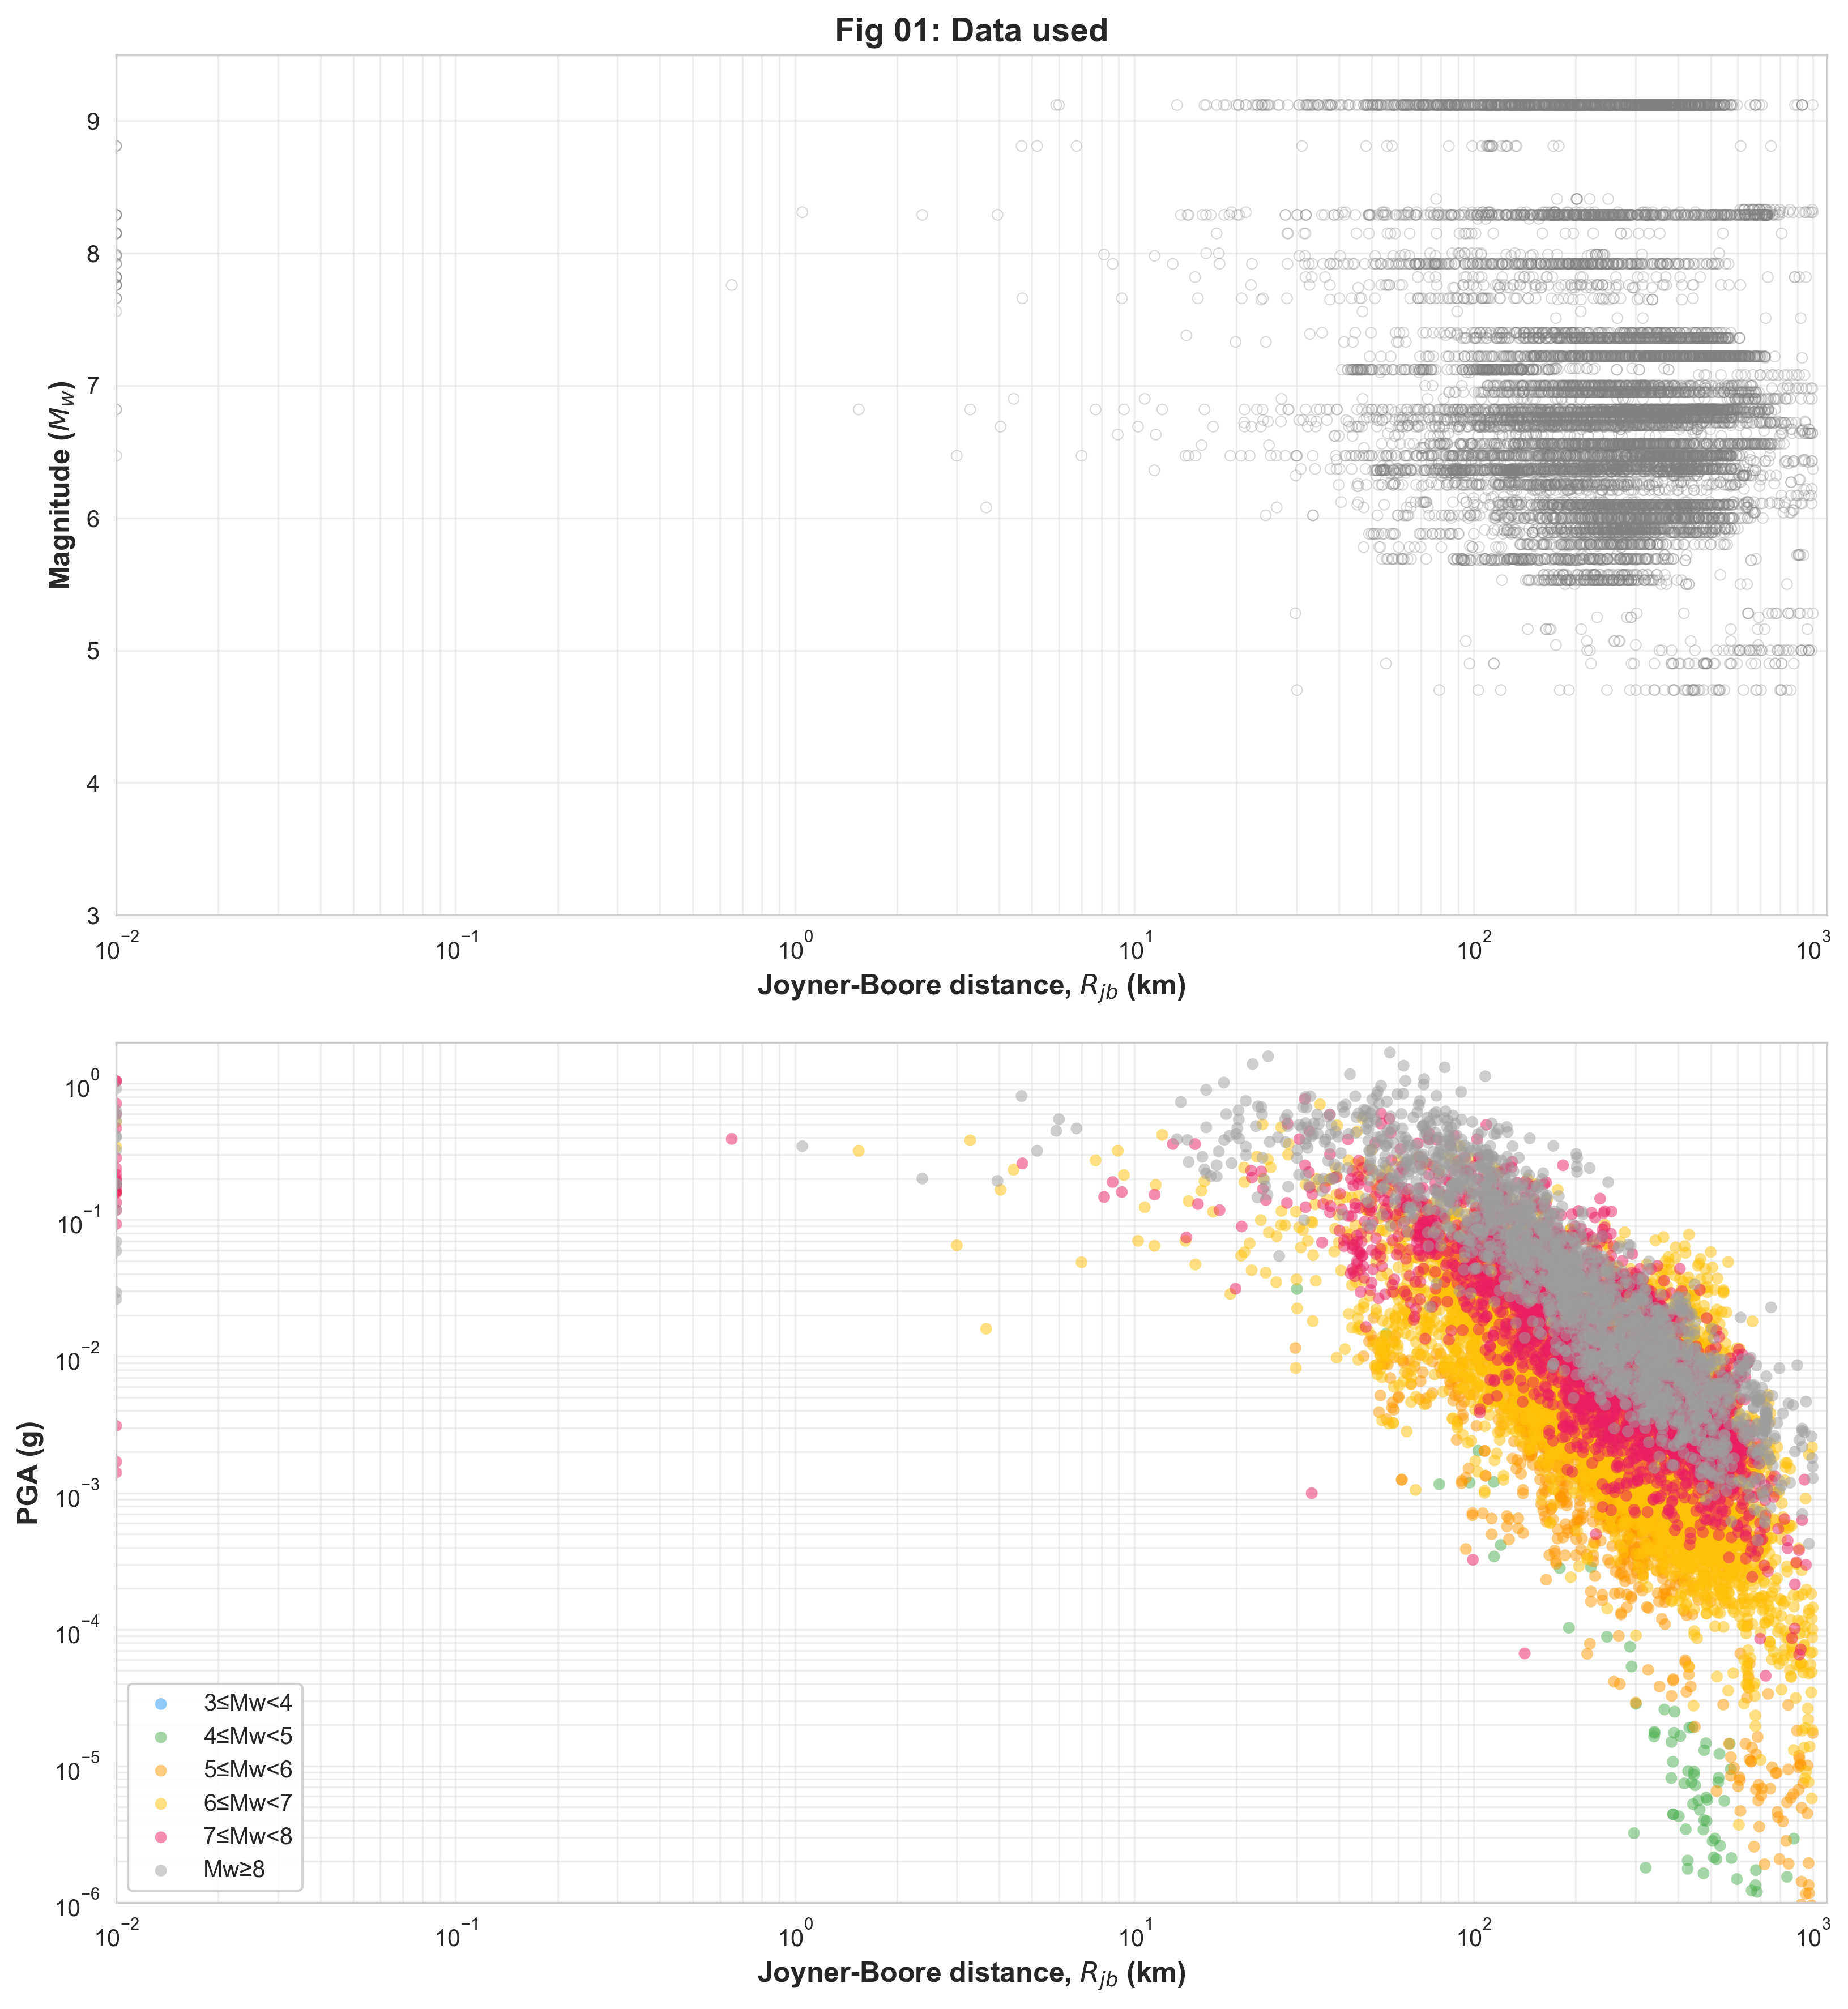
\includegraphics[width=0.95\linewidth]{fig01_data_distribution}
  \caption{NGA-Subduction dataset distribution after cleaning (13{,}495 records).
           Scatter plots show $M_w$ vs.\ $R_{jb}$, $V_{s30}$, and $Z_{tor}$,
           coloured by focal mechanism.}
  \label{fig:data_dist}
\end{figure}

\begin{figure}[htbp]
  \centering
  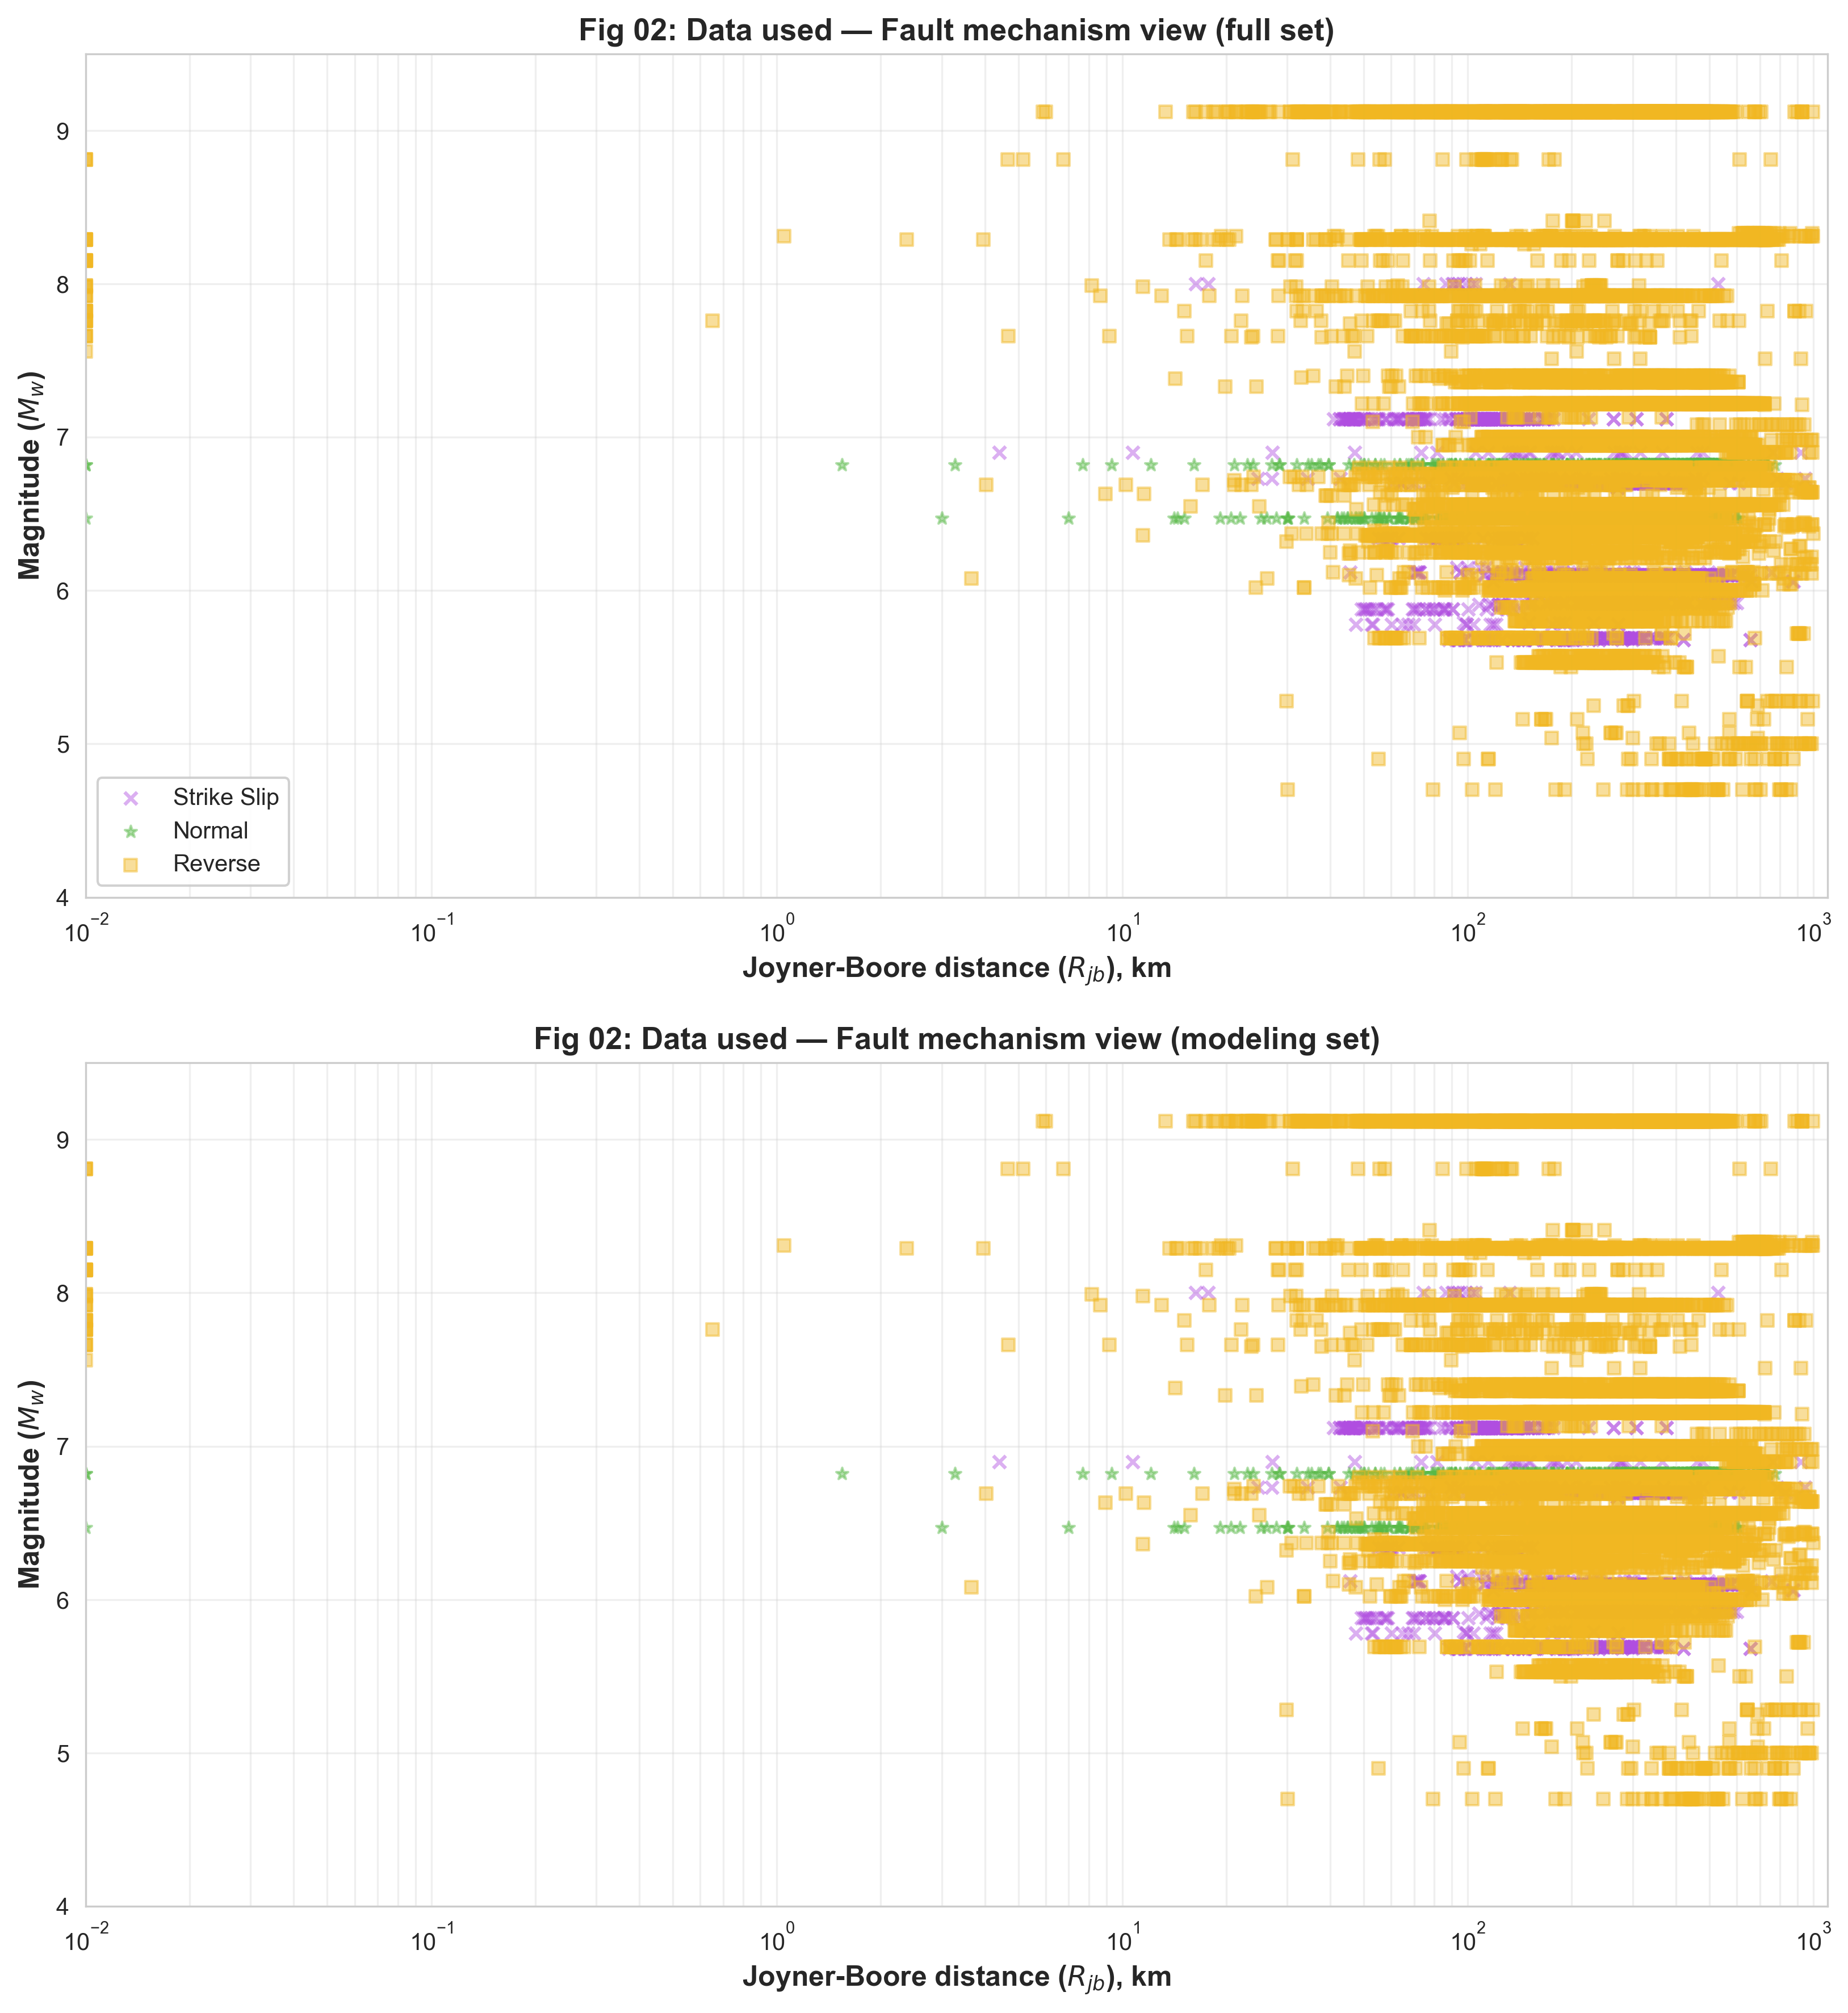
\includegraphics[width=0.95\linewidth]{fig02_data_used}
  \caption{Distribution of records by focal mechanism (Strike-Slip, Normal,
           Reverse) and across the predictor space.}
  \label{fig:data_used}
\end{figure}

\begin{figure}[htbp]
  \centering
  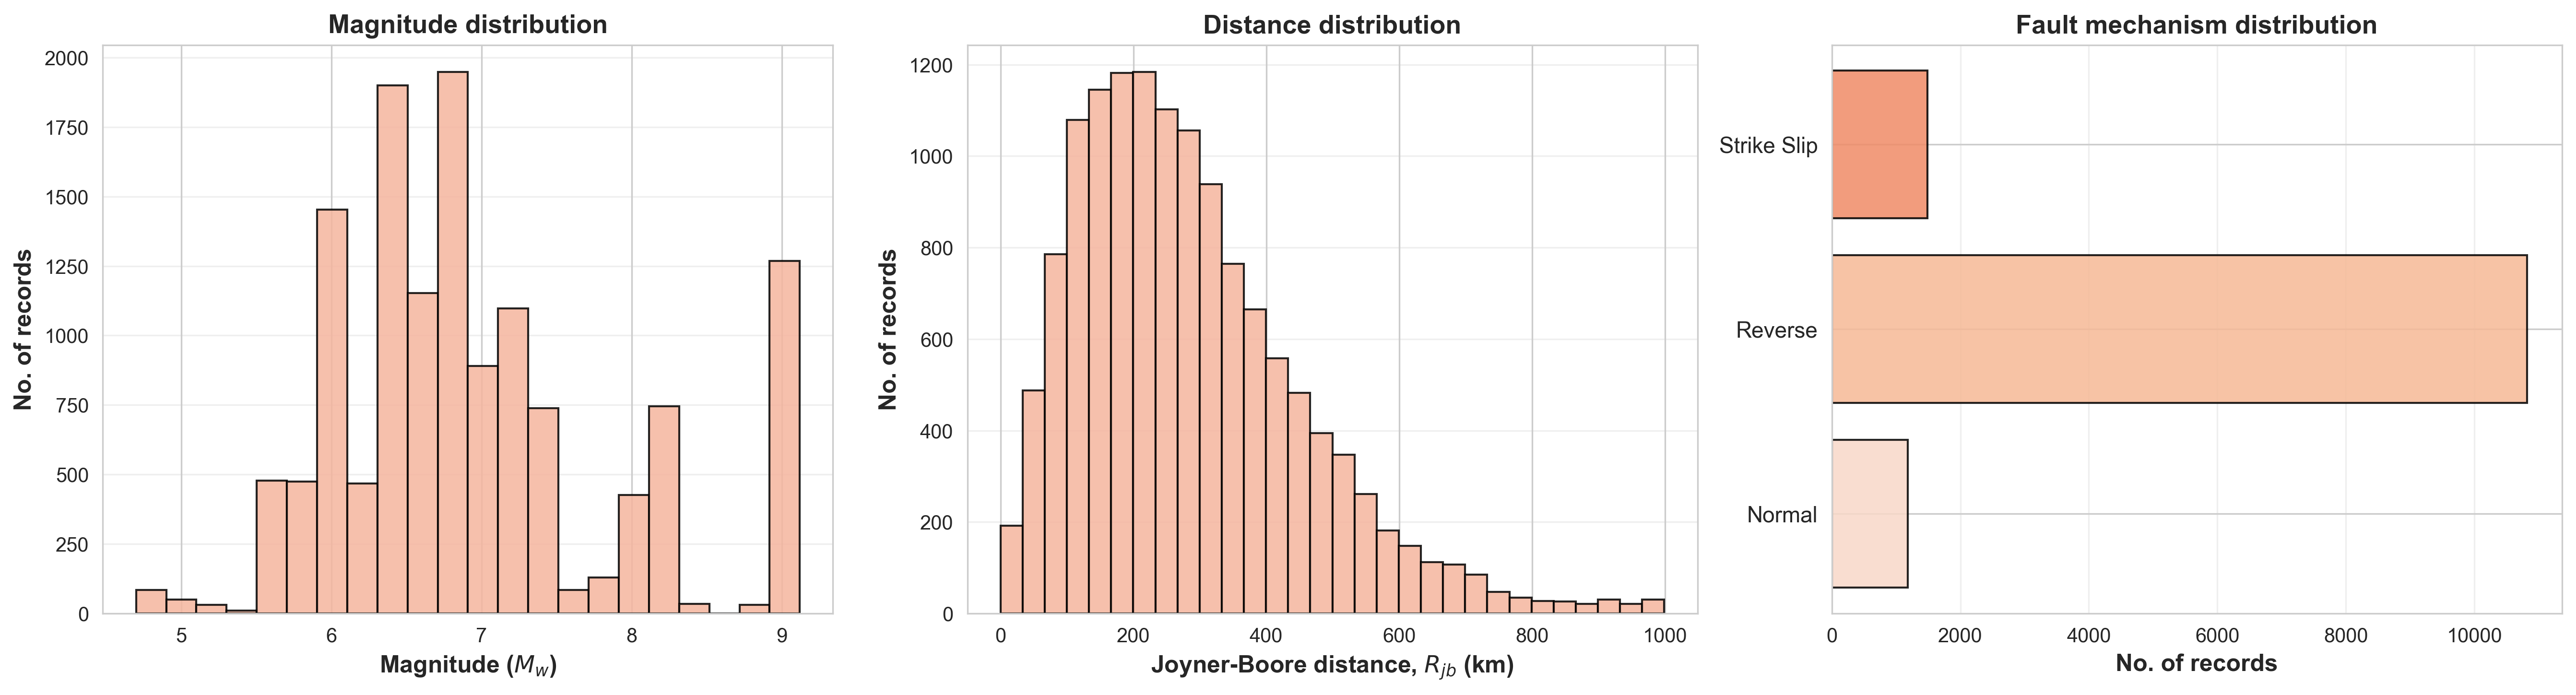
\includegraphics[width=0.95\linewidth]{fig03_frequency_plots}
  \caption{Univariate frequency distributions of the eight input features and
           key target IMs in the training set.}
  \label{fig:freq}
\end{figure}

% ===================================================================
%  4. MODEL ARCHITECTURE
% ===================================================================
\section{BiLSTM-GMM Architecture}
\label{sec:arch}

Figure~\ref{fig:arch} illustrates the overall architecture.
The model takes as input a single earthquake--site feature vector
$\mathbf{x} \in \mathbb{R}^8$ and produces $K = 30$ log-IM predictions
$\hat{\mathbf{y}} = (\hat{y}_1, \ldots, \hat{y}_K)$ in a single forward pass.

\begin{figure}[htbp]
  \centering
  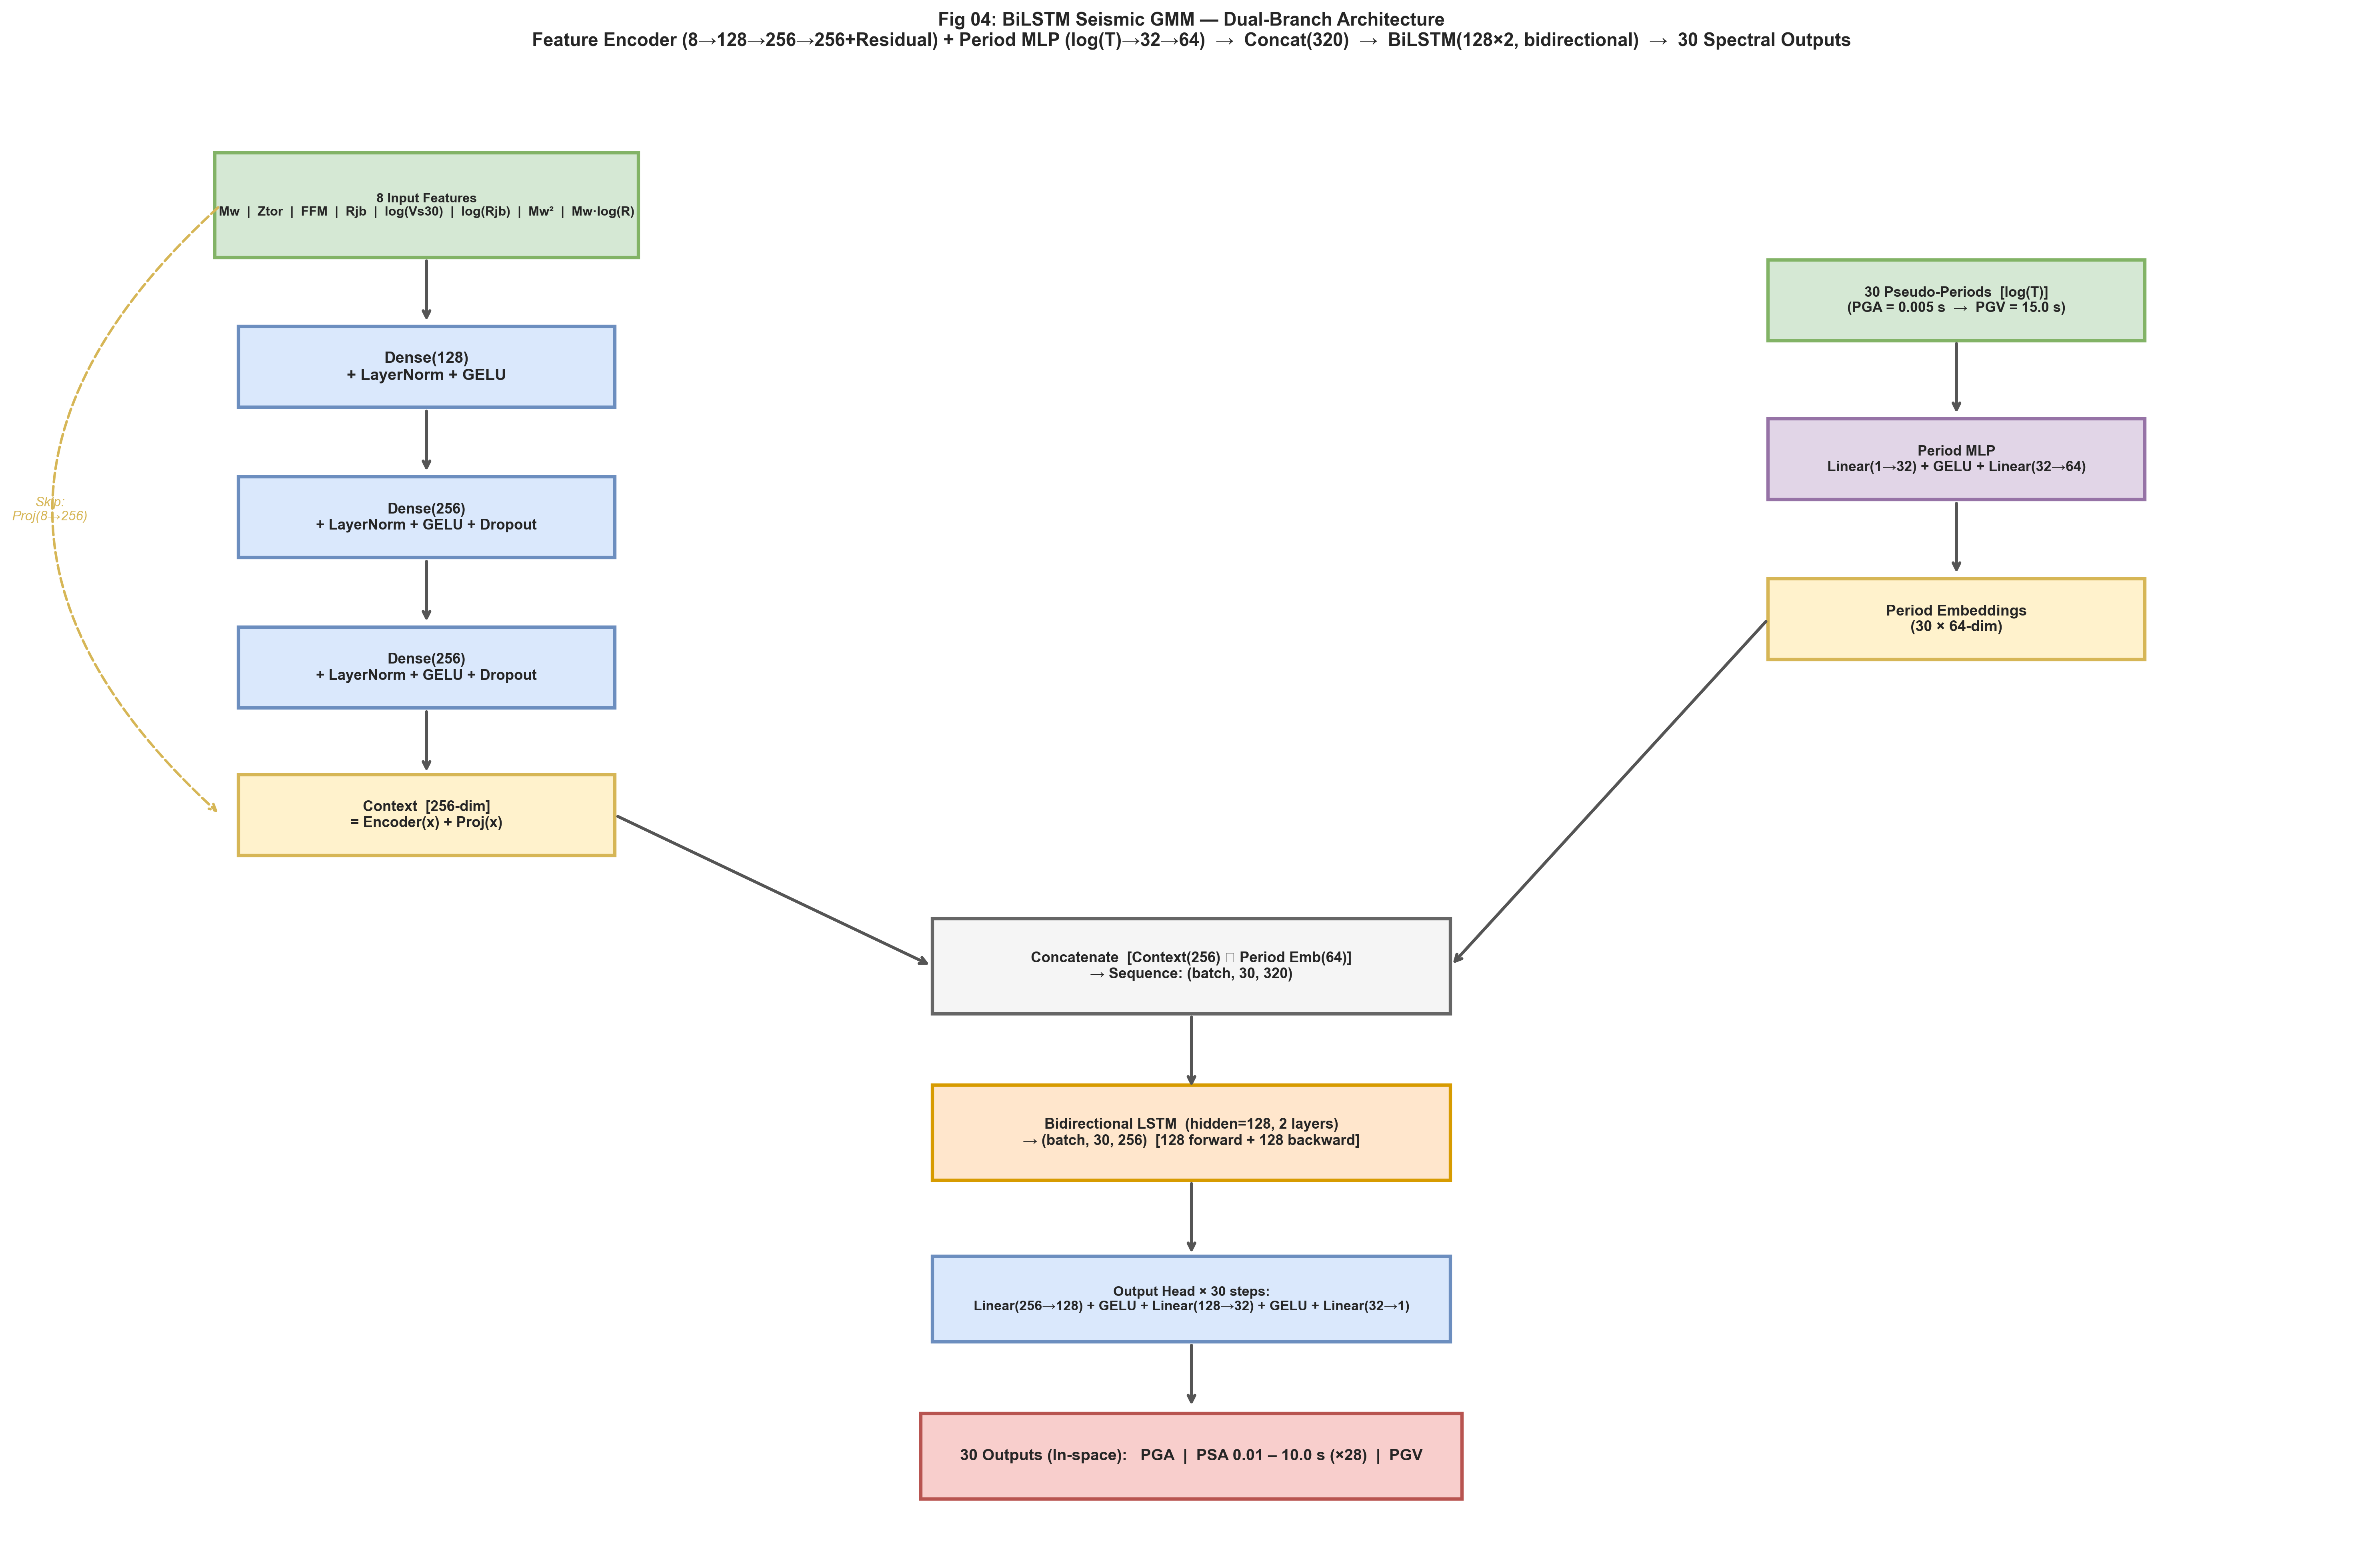
\includegraphics[width=\linewidth]{fig04_architecture}
  \caption{BiLSTM-GMM dual-branch architecture.
           The Feature Encoder (left branch, blue/green boxes) maps the
           8-dimensional input to a 256-dimensional context vector using a
           residual MLP.
           The Period Embedding MLP (right branch, purple box) maps each
           log-pseudo-period $\ln T_k$ to a 64-dimensional embedding.
           Concatenated representations form the BiLSTM input sequence
           ($\mathbb{R}^{320}$ per step), and the Output Head projects each
           BiLSTM hidden state to a scalar log-IM prediction.}
  \label{fig:arch}
\end{figure}

\subsection{Feature Encoder with Residual Projection}

Let $\mathbf{x} \in \mathbb{R}^{N_x}$ ($N_x = 8$) be the input feature vector.
All features are standardised to zero mean and unit variance using statistics
computed from the training set only.
The Feature Encoder maps $\mathbf{x}$ to a context vector
$\mathbf{c} \in \mathbb{R}^{d_c}$ ($d_c = 256$) via:
\begin{equation}
  \mathbf{c} = \mathrm{Enc}_\theta(\mathbf{x}) + \mathbf{W}_\mathrm{skip}\,\mathbf{x}
  \label{eq:encoder}
\end{equation}
where $\mathbf{W}_\mathrm{skip} \in \mathbb{R}^{d_c \times N_x}$ is a learned
linear projection (no bias) that implements a residual skip connection.
The encoder $\mathrm{Enc}_\theta$ consists of five fully connected blocks:
\begin{equation}
  \mathrm{Enc}_\theta:
  \mathbb{R}^{8} \xrightarrow{\mathrm{FC}_{128}} \to
  \xrightarrow{\mathrm{FC}_{256}} \to
  \xrightarrow{\mathrm{FC}_{512}} \to
  \xrightarrow{\mathrm{FC}_{512}} \to
  \xrightarrow{\mathrm{FC}_{256}}
  \mathbb{R}^{256}
\end{equation}
Each $\mathrm{FC}_{d}$ block applies a linear transform, Layer Normalisation
\citep{Ba2016}, GELU activation \citep{Hendrycks2016}, and Dropout (rate 0.2,
omitted in the first block to preserve gradient flow).
The residual connection bypasses the depth of the encoder, mitigating vanishing
gradients and accelerating convergence \citep{He2016}.

\subsection{Continuous Period Embedding}
\label{sec:period_embed}

Each of the $K=30$ output slots is associated with a pseudo-period $T_k$.
Rather than one-hot encoding or a lookup table (which would not generalise to
unseen periods), we use a continuous MLP:
\begin{equation}
  \mathbf{p}_k = g_\phi(\ln T_k), \quad
  g_\phi: \mathbb{R}^1 \xrightarrow{\mathrm{FC}_{32}} \to
          \xrightarrow{\mathrm{FC}_{64}} \mathbb{R}^{d_p}
  \label{eq:period_embed}
\end{equation}
with $d_p = 64$ and GELU activations.
Using $\ln T_k$ as input reflects the physical convention that spectral
ordinates vary smoothly in log-period space.
The log-period values are registered as a fixed buffer in the model (not
trainable), preserving correct ordering for the BiLSTM.
PGA is assigned $\ln(0.005)$ and PGV $\ln(15)$, situating them at the ends of
the spectral sequence.

\subsection{Sequence Fusion and Bidirectional LSTM}

For each period step $k$, the context vector $\mathbf{c}$ is concatenated with
the period embedding $\mathbf{p}_k$ to form the BiLSTM input:
\begin{equation}
  \mathbf{s}_k = [\mathbf{c};\, \mathbf{p}_k] \in \mathbb{R}^{d_c + d_p = 320},
  \quad k = 1, \ldots, K.
  \label{eq:fusion}
\end{equation}
The sequence $(\mathbf{s}_1, \ldots, \mathbf{s}_K)$ is processed by a
two-layer bidirectional LSTM \citep{Schuster1997}:
\begin{align}
  \overrightarrow{\mathbf{h}}_k &= \overrightarrow{\mathrm{LSTM}}(\mathbf{s}_k,
    \overrightarrow{\mathbf{h}}_{k-1}),
    \quad \overrightarrow{\mathbf{h}}_k \in \mathbb{R}^{d_h},\\
  \overleftarrow{\mathbf{h}}_k &= \overleftarrow{\mathrm{LSTM}}(\mathbf{s}_k,
    \overleftarrow{\mathbf{h}}_{k+1}),
    \quad \overleftarrow{\mathbf{h}}_k \in \mathbb{R}^{d_h},\\
  \mathbf{h}_k &= [\overrightarrow{\mathbf{h}}_k;\, \overleftarrow{\mathbf{h}}_k]
    \in \mathbb{R}^{2d_h},
  \label{eq:bilstm}
\end{align}
with hidden size $d_h = 256$ per direction (512 total), 2 layers, and inter-layer
dropout rate 0.2.
The forward pass propagates spectral information from short to long periods,
while the backward pass propagates it in the opposite direction, enabling the
model to encode both the high-frequency spectral plateau (controlled by
magnitude and near-field distance) and the long-period spectral corner
(controlled by rupture area and low-$V_{s30}$ site amplification).

\subsection{Output Head}

A shared output head projects each per-step hidden state
$\mathbf{h}_k \in \mathbb{R}^{512}$ to a scalar log-IM prediction:
\begin{equation}
  \hat{y}_k =
  \mathrm{Linear}(32, 1) \circ \mathrm{GELU} \circ
  \mathrm{Linear}(128, 32) \circ \mathrm{GELU} \circ
  \mathrm{Dropout}(0.1) \circ
  \mathrm{Linear}(512, 128)\,(\mathbf{h}_k).
  \label{eq:output_head}
\end{equation}
Target log-IM values are standardised using training-set statistics
(mean and standard deviation computed jointly across all 30 outputs);
predictions are inverse-transformed before loss computation.

\subsection{Parameter Count}

The model contains \textbf{998{,}593 trainable parameters}, distributed as:
feature encoder $\approx$440k, residual projection $\approx$2k, period
embedding $\approx$2k, BiLSTM $\approx$526k, and output head $\approx$27k.

\subsection{End-to-End Prediction Pipeline}
\label{sec:pipeline}

This subsection traces a single prediction from raw earthquake and site
parameters to physical IM values, making the full mathematical logic
explicit.

\paragraph{Step 1 — Physics-informed feature construction.}
Given raw inputs $(M_w, Z_{tor}, \text{FFM}, R_{jb}, V_{s30})$, the
eight-dimensional feature vector is assembled as:
\begin{equation}
  \mathbf{x} = \bigl[
    M_w,\;
    Z_{tor},\;
    \text{FFM},\;
    R_{jb},\;
    \ln V_{s30},\;
    \ln\!\max(R_{jb},\,0.1),\;
    M_w^2,\;
    M_w\cdot\ln\!\max(R_{jb},\,0.1)
  \bigr]^{\!\top} \in \mathbb{R}^8.
  \label{eq:features}
\end{equation}
The floor $\max(R_{jb}, 0.1\,\text{km})$ prevents $-\infty$ for on-fault
records.
$\ln V_{s30}$ linearises the well-known log-linear site amplification
relationship; $M_w^2$ captures magnitude-squared scaling (amplitude
saturation); and $M_w\cdot\ln R_{jb}$ encodes the physical principle that
stronger earthquakes maintain high ground motion over longer path lengths.

\paragraph{Step 2 — Input standardisation.}
Every feature is standardised to zero mean and unit variance using statistics
$(\boldsymbol{\mu}_x, \boldsymbol{\sigma}_x)$ computed from the training set:
\begin{equation}
  \tilde{x}_i = \frac{x_i - \mu_{x,i}}{\sigma_{x,i}}, \quad i = 1,\ldots,8.
  \label{eq:standardise_x}
\end{equation}

\paragraph{Step 3 — Dual-branch forward pass.}
The standardised vector $\tilde{\mathbf{x}}$ enters the Feature Encoder
with residual skip (Eq.~\ref{eq:encoder}), yielding context
$\mathbf{c}\in\mathbb{R}^{256}$.
For each of the $K=30$ spectral steps the Period Embedding MLP maps
$\ln T_k$ to $\mathbf{p}_k\in\mathbb{R}^{64}$ (Eq.~\ref{eq:period_embed}).
The fused sequence
$(\mathbf{s}_1,\ldots,\mathbf{s}_K)$, $\mathbf{s}_k=[\mathbf{c};\mathbf{p}_k]$
(Eq.~\ref{eq:fusion}),
is processed by the BiLSTM (Eq.~\ref{eq:bilstm}), and the Output Head
(Eq.~\ref{eq:output_head}) maps each hidden state
$\mathbf{h}_k\in\mathbb{R}^{512}$ to a scalar:
\begin{equation}
  \hat{z}_k = \mathrm{OutputHead}(\mathbf{h}_k) \in \mathbb{R},
  \quad k = 1,\ldots,30.
  \label{eq:scaled_output}
\end{equation}

\paragraph{Step 4 — Output inverse standardisation.}
Targets were standardised jointly across all 30 outputs using training-set
statistics $(\mu_{y,k}, \sigma_{y,k})$ (computed in $\ln$-IM space).
The network prediction $\hat{z}_k$ is therefore in scaled $\ln$-IM space;
it is recovered as:
\begin{equation}
  \hat{y}_k^{(\ln)} = \sigma_{y,k}\,\hat{z}_k + \mu_{y,k},
  \label{eq:inv_scale_y}
\end{equation}
where $\hat{y}_k^{(\ln)}$ is the predicted natural logarithm of the $k$-th IM.

\paragraph{Step 5 — Exponentiation to physical units.}
\begin{equation}
  \widehat{\mathrm{IM}}_k = \exp\!\bigl(\hat{y}_k^{(\ln)}\bigr),
  \quad
  \begin{cases}
    k = 0: & \widehat{\mathrm{PGA}}\ [\text{g}] \\
    k = 1,\ldots,28: & \widehat{\mathrm{PSA}}(T_k)\ [\text{g}] \\
    k = 29: & \widehat{\mathrm{PGV}}\ [\text{cm/s}]
  \end{cases}
  \label{eq:exponentiate}
\end{equation}

\paragraph{Compact end-to-end formula.}
Combining Steps~1--5, the complete BiLSTM-GMM prediction for the $k$-th IM is:
\begin{equation}
  \boxed{
    \widehat{\mathrm{IM}}_k(M_w, R_{jb}, V_{s30}, Z_{tor}, \text{FFM})
    = \exp\!\Bigl(
        \sigma_{y,k}\cdot
        h_k\bigl(
          \mathrm{Enc}(\tilde{\mathbf{x}}) + \mathbf{W}_\text{skip}\tilde{\mathbf{x}},\;
          g_\phi(\ln T_k)
        \bigr)
        + \mu_{y,k}
      \Bigr)
  }
  \label{eq:full_model}
\end{equation}
where $h_k(\cdot)$ denotes the BiLSTM + Output Head applied at step $k$.
The model is \emph{median-predicting}: Eq.~\ref{eq:full_model} returns
$e^{\hat{\mu}_k}$, the geometric-mean prediction.
Aleatory variability around the median is characterised by the total sigma
$\sigma_T$ reported in Table~\ref{tab:sigma}; the full log-normal distribution
of any IM given the inputs is therefore $\ln\text{IM}_k \sim
\mathcal{N}(\hat{y}_k^{(\ln)},\,\sigma_{T,k}^2)$.

Algorithm~\ref{alg:predict} summarises the prediction procedure for practitioners.

\begin{algorithm}[htbp]
\caption{BiLSTM-GMM single-scenario prediction}
\label{alg:predict}
\begin{algorithmic}[1]
\Require $M_w, R_{jb}\ [\text{km}], V_{s30}\ [\text{m/s}], Z_{tor}\ [\text{km}],
         \text{FFM}\in\{0,1\}$
\Require Trained weights $\theta$; scalers $(\boldsymbol{\mu}_x,\boldsymbol{\sigma}_x)$,
         $(\boldsymbol{\mu}_y,\boldsymbol{\sigma}_y)$
\State $\mathbf{x} \leftarrow [M_w,\;Z_{tor},\;\text{FFM},\;R_{jb},\;\ln V_{s30},\;
        \ln\!\max(R_{jb},0.1),\;M_w^2,\;M_w\!\cdot\!\ln\!\max(R_{jb},0.1)]$
\State $\tilde{\mathbf{x}} \leftarrow (\mathbf{x}-\boldsymbol{\mu}_x)/\boldsymbol{\sigma}_x$
\State $\mathbf{c} \leftarrow \mathrm{Enc}_\theta(\tilde{\mathbf{x}}) +
        \mathbf{W}_\text{skip}\tilde{\mathbf{x}}$ \Comment{Feature context, 256-dim}
\For{$k = 1$ \textbf{to} $30$}
  \State $\mathbf{p}_k \leftarrow g_\phi(\ln T_k)$ \Comment{Period embedding, 64-dim}
  \State $\mathbf{s}_k \leftarrow [\mathbf{c};\,\mathbf{p}_k]$ \Comment{Concat, 320-dim}
\EndFor
\State $(\mathbf{h}_1,\ldots,\mathbf{h}_{30}) \leftarrow
        \mathrm{BiLSTM}_\theta(\mathbf{s}_1,\ldots,\mathbf{s}_{30})$
\For{$k = 1$ \textbf{to} $30$}
  \State $\hat{z}_k \leftarrow \mathrm{OutputHead}_\theta(\mathbf{h}_k)$
  \State $\hat{y}_k^{(\ln)} \leftarrow \sigma_{y,k}\,\hat{z}_k + \mu_{y,k}$
  \State $\widehat{\mathrm{IM}}_k \leftarrow \exp(\hat{y}_k^{(\ln)})$
\EndFor
\State \Return $(\widehat{\mathrm{IM}}_1,\ldots,\widehat{\mathrm{IM}}_{30})$ \Comment{PGA, PSA$\times$28, PGV}
\end{algorithmic}
\end{algorithm}

% ===================================================================
%  5. TRAINING PROCEDURE
% ===================================================================
\section{Training Procedure}
\label{sec:training}

\subsection{Loss Function}

The training objective combines a robust loss and a physics-motivated
spectral regulariser:
\begin{equation}
  \mathcal{L} = \mathcal{L}_{\mathrm{Huber}} + \lambda\,\mathcal{L}_{\mathrm{smooth}}
  \label{eq:loss}
\end{equation}

\paragraph{Huber loss.}
\begin{equation}
  \mathcal{L}_{\mathrm{Huber}} = \frac{1}{NK}\sum_{n=1}^{N}\sum_{k=1}^{K}
  L_\delta(\hat{y}_{n,k},\, y_{n,k}), \qquad
  L_\delta(a,b) =
  \begin{cases}
    \tfrac{1}{2}(a-b)^2 & |a-b| \le \delta \\
    \delta\bigl(|a-b| - \tfrac{\delta}{2}\bigr) & \text{otherwise}
  \end{cases}
  \label{eq:huber}
\end{equation}
with $\delta = 0.5$ (in scaled log-IM units).
The Huber loss reduces sensitivity to outlier records without discarding their
information entirely, which is important for the heavy tails present in
log-normal ground motion distributions.

\paragraph{Spectral smoothness regulariser.}
Physical response spectra are smooth in log-period space.
We penalise second-order finite differences of the predicted log-IM sequence
to enforce this:
\begin{equation}
  \mathcal{L}_{\mathrm{smooth}} = \frac{1}{N(K{-}2)}\sum_{n=1}^{N}
  \sum_{k=2}^{K-1}
  \bigl(\hat{y}_{n,k+1} - 2\hat{y}_{n,k} + \hat{y}_{n,k-1}\bigr)^2
  \label{eq:smooth}
\end{equation}
with regularisation weight $\lambda = 5 \times 10^{-4}$.
This curvature penalty discourages spectral humps or notches at individual
periods---a known failure mode when models have high local flexibility.

\subsection{Optimiser and Learning Rate Schedule}

The AdamW optimiser \citep{Loshchilov2019} is used with initial learning rate
$\eta_0 = 2 \times 10^{-3}$ and weight decay $\lambda_w = 10^{-4}$.
The one-cycle learning rate policy \citep{Smith2019} is applied per batch:
the rate warms up from $\eta_0/25$ to $\eta_0$ over the first 30\% of
training steps (pct\_start~$= 0.30$), then decays to near zero via cosine
annealing.
This schedule has been shown to enable faster convergence and better
generalisation than fixed-rate or step-decay schedules
\citep{Smith2019}.

\subsection{Training Details}

\begin{table}[htbp]
\centering
\caption{Training hyperparameters.}
\label{tab:hparams}
\footnotesize
\renewcommand{\arraystretch}{1.15}
\begin{tabular}{ll}
\toprule
Hyperparameter & Value \\
\midrule
Optimiser & AdamW \\
Initial learning rate $\eta_0$ & $2 \times 10^{-3}$ \\
Weight decay $\lambda_w$ & $1 \times 10^{-4}$ \\
Batch size & 256 \\
Maximum epochs & 150 \\
Early-stopping patience & 30 epochs \\
LR schedule & OneCycleLR (max\_lr $= 2\times10^{-3}$, pct\_start $= 0.30$, cosine anneal) \\
Huber $\delta$ & 0.5 \\
Smoothness weight $\lambda$ & $5 \times 10^{-4}$ \\
Dropout (Encoder) & 0.20 \\
Dropout (Output Head) & 0.10 \\
Activation & GELU \\
Normalisation & Layer Normalisation \\
Residual skip & Yes \\
Period encoding & Continuous $\ln T$ MLP \\
Hardware & CPU (Intel/AMD, no GPU) \\
\bottomrule
\end{tabular}
\end{table}

Training was terminated at epoch~\textbf{87} by early stopping (patience~30),
with best validation Huber loss $= 0.0596$.
All computations were performed in IEEE 32-bit floating point with PyTorch 2.x.
Random seeds were fixed (seed~42) for reproducibility.

% ===================================================================
%  6. RESULTS AND EVALUATION
% ===================================================================
\section{Results and Evaluation}
\label{sec:results}

\subsection{Overall Performance}
\label{sec:overall}

Table~\ref{tab:overall} reports aggregate $R^2$, RMSE, and MAE (all in
natural-log units) across all 30 output IMs on the training, validation, and
test sets.
The small gap between training ($R^2 = 0.935$) and test ($R^2 = 0.925$)
performance confirms that generalisation is achieved without overfitting.

\begin{table}[htbp]
\centering
\caption{Aggregate performance metrics (natural-log units, all 30 IMs).}
\label{tab:overall}
\footnotesize
\renewcommand{\arraystretch}{1.15}
\begin{tabular}{lcccc}
\toprule
Split & $N$ & $R^2$ & RMSE (ln) & MAE (ln) \\
\midrule
Training   & 9{,}451 & 0.935 & 0.620 & 0.463 \\
Validation & 2{,}019 & 0.919 & 0.683 & 0.520 \\
\textbf{Test} & \textbf{2{,}025} & \textbf{0.925} & \textbf{0.673} & \textbf{0.510} \\
\bottomrule
\end{tabular}
\end{table}

\subsection{Per-Intensity-Measure Performance}
\label{sec:per_im}

Table~\ref{tab:per_im} reports Pearson correlation $r$ and coefficient of
determination $R^2$ for 12 representative IMs on the test set.
Per-IM $r$ ranges from 0.916 (PSA at 2~s) to 0.956 (PSA at 10~s and PGV),
with all IMs exceeding $r = 0.924$.
The slight dip at 2~s reflects the transition region between source-dominated
and site-dominated spectral behaviour, where aleatory variability is
intrinsically highest.

\begin{table}[htbp]
\centering
\caption{Per-IM test-set performance for representative intensity measures.
Full results for all 30 IMs are available in the supplementary data.}
\label{tab:per_im}
\footnotesize
\renewcommand{\arraystretch}{1.15}
\begin{tabular}{lcccc}
\toprule
IM & Period (s) & $r$ & $R^2$ & RMSE (ln) \\
\midrule
PGA        & 0.005 (pseudo) & 0.939 & 0.882 & 0.655 \\
PSA(0.01s) & 0.01           & 0.939 & 0.881 & 0.657 \\
PSA(0.1s)  & 0.10           & 0.924 & 0.853 & 0.778 \\
PSA(0.2s)  & 0.20           & 0.927 & 0.858 & 0.768 \\
PSA(0.3s)  & 0.30           & 0.934 & 0.873 & 0.709 \\
PSA(0.5s)  & 0.50           & 0.936 & 0.876 & 0.664 \\
PSA(1.0s)  & 1.00           & 0.927 & 0.860 & 0.664 \\
PSA(2.0s)  & 2.00           & 0.916 & 0.839 & 0.716 \\
PSA(3.0s)  & 3.00           & 0.923 & 0.852 & 0.705 \\
PSA(5.0s)  & 5.00           & 0.939 & 0.882 & 0.646 \\
PSA(10s)   & 10.0           & \textbf{0.956} & \textbf{0.912} & 0.577 \\
PGV        & 15.0 (pseudo)  & \textbf{0.954} & \textbf{0.910} & 0.546 \\
\bottomrule
\end{tabular}
\end{table}

Figure~\ref{fig:regression} shows predicted-versus-observed scatter plots for
PGA, PSA(0.1s), PSA(1.0s), and PGV.
Points lie tightly along the 1:1 line across five orders of magnitude,
confirming unbiased predictions.

\begin{figure}[htbp]
  \centering
  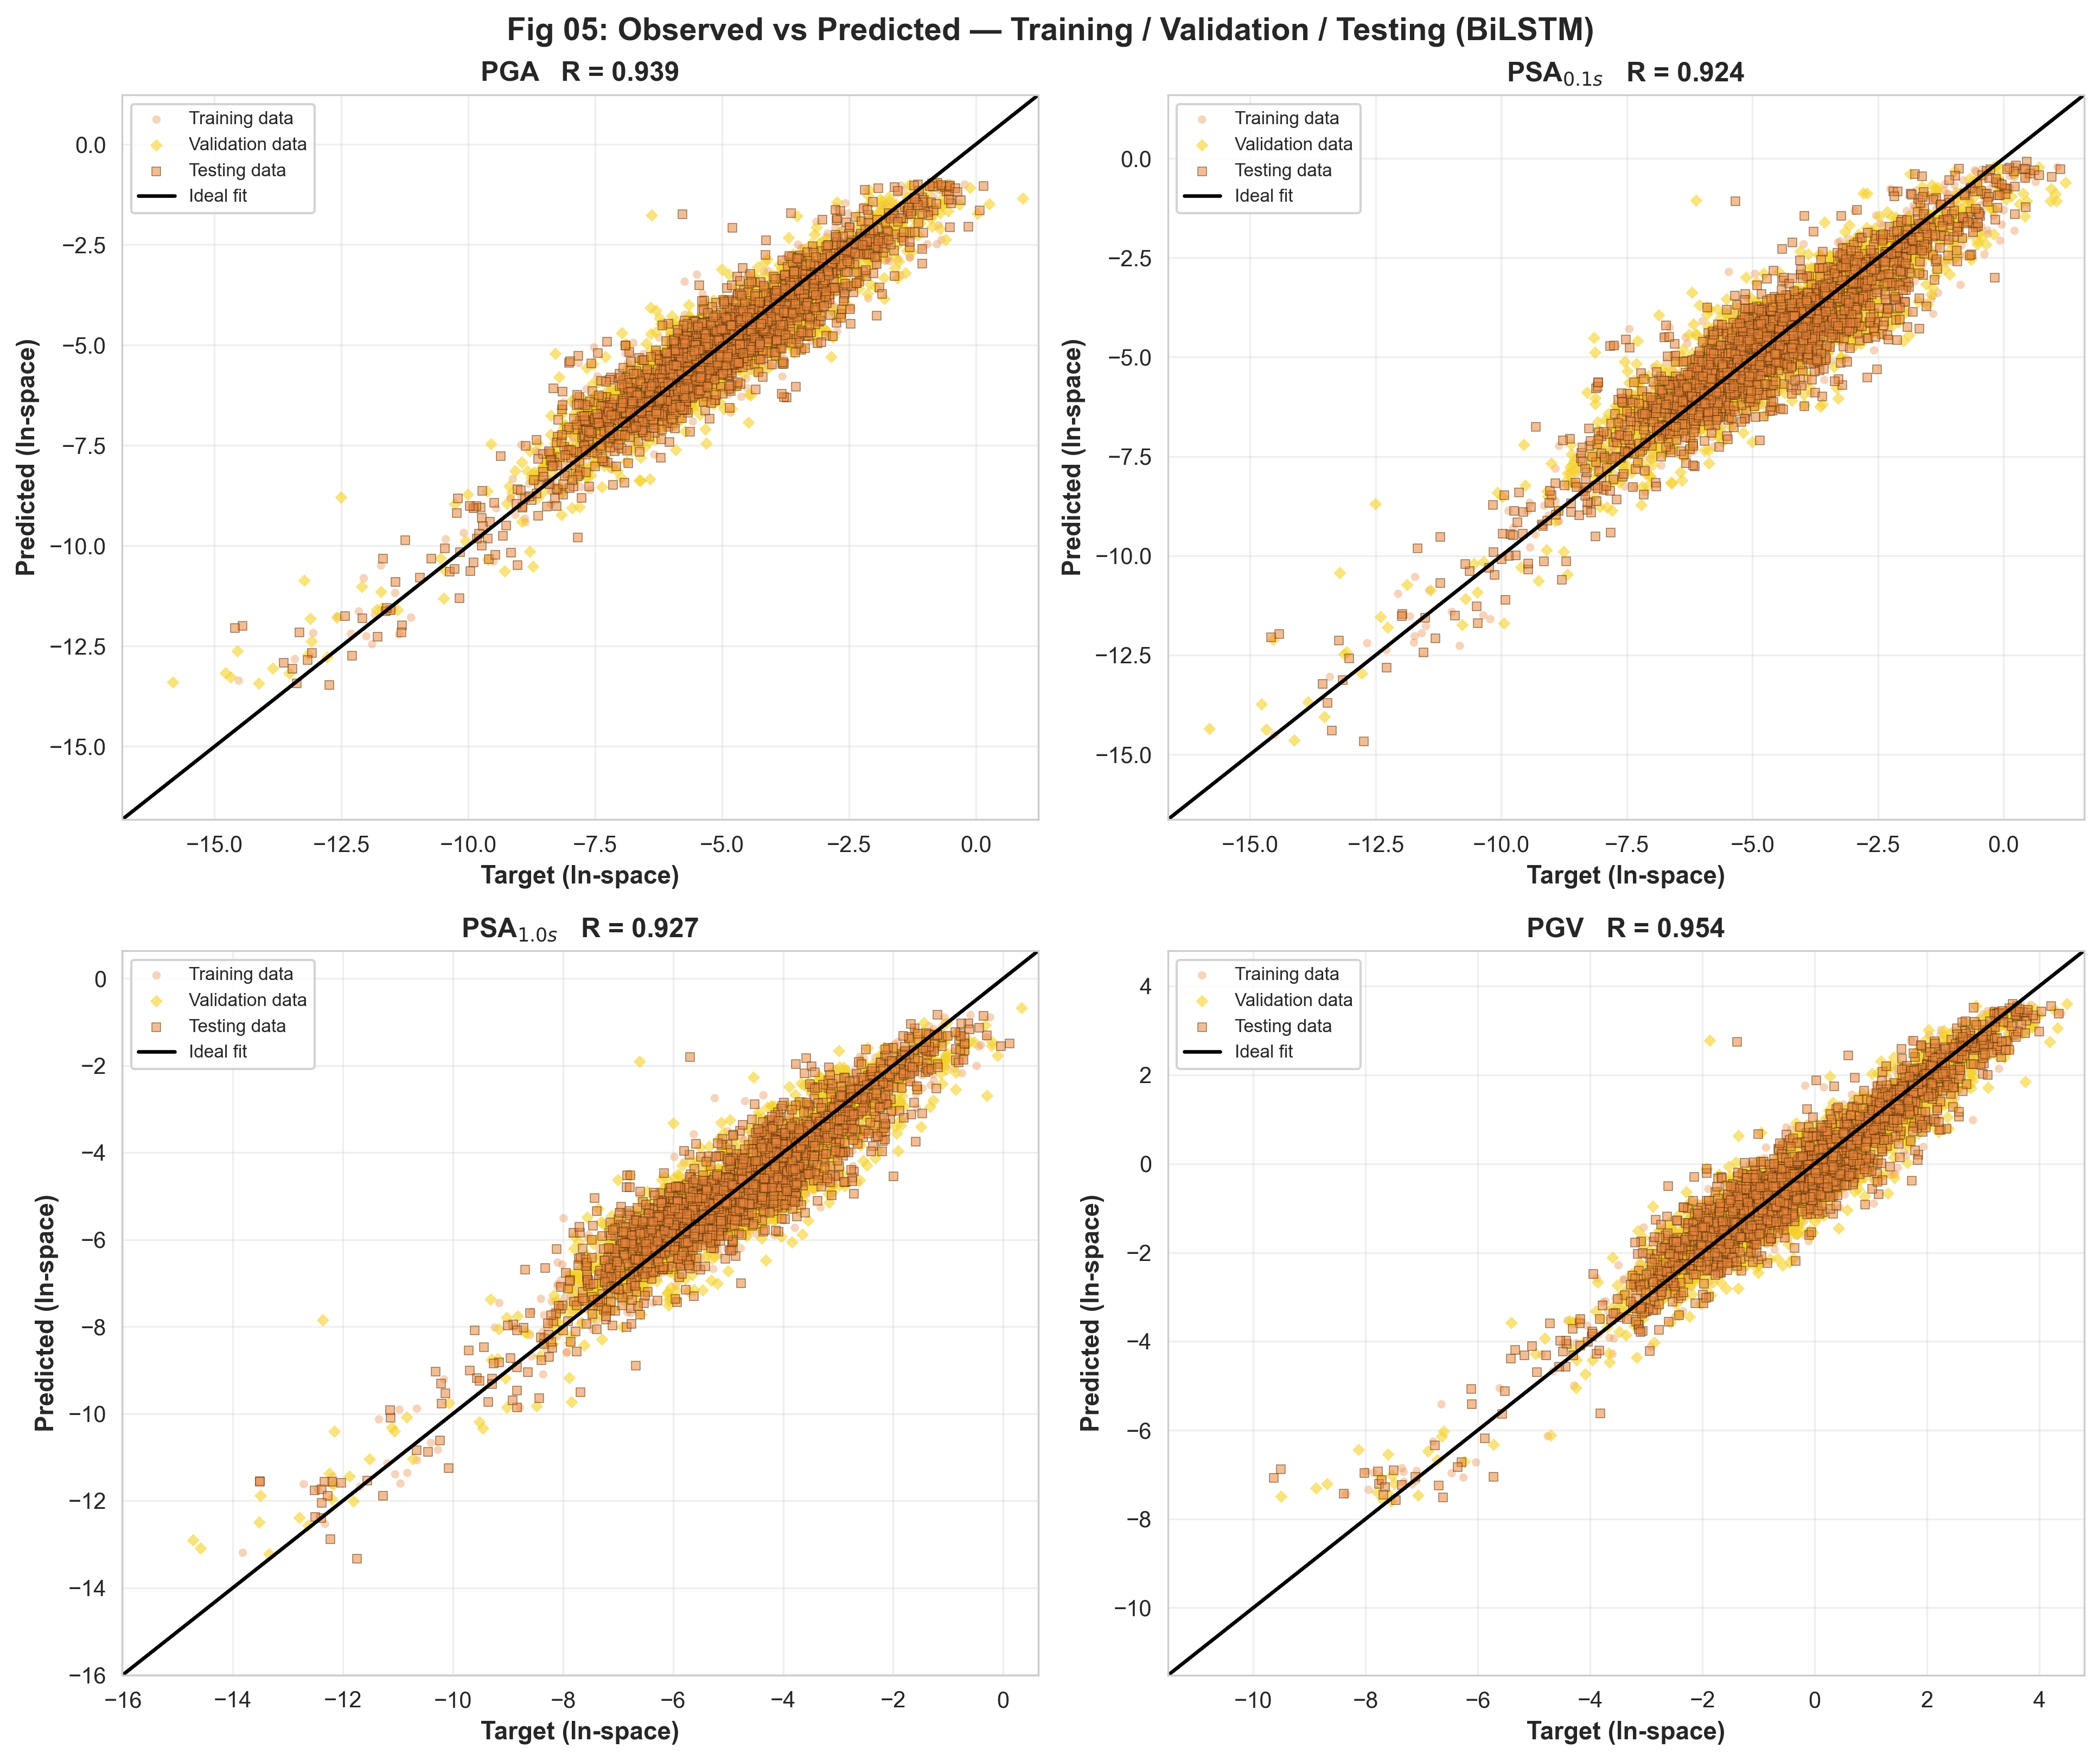
\includegraphics[width=\linewidth]{fig05_regression_plots}
  \caption{Predicted vs.\ observed (natural-log scale) for PGA, PSA(0.1s),
           PSA(1.0s), and PGV on the held-out test set ($N=2{,}025$).
           The dashed line indicates the 1:1 reference; $r$ and RMSE values
           are annotated in each panel.}
  \label{fig:regression}
\end{figure}

\subsection{Residual Analysis}
\label{sec:residuals}

Figure~\ref{fig:residuals} shows total residuals
$\varepsilon = \ln\text{IM}_\text{obs} - \ln\text{IM}_\text{pred}$
plotted against $M_w$, $R_{jb}$, and $\ln V_{s30}$ for PGA, PSA(0.1s),
PSA(1.0s), and PSA(4.0s).
Residuals are mean-centred (global mean subtracted) and binned; error bars
show $\pm 1$ standard deviation within each bin.
No systematic trends are visible in magnitude or distance, confirming that the
model has absorbed the primary scaling behaviours.
A slight increase in scatter at very high $V_{s30}$ (hard rock) reflects the
limited number of hard-rock recordings in the NGA-Subduction dataset.

\begin{figure}[htbp]
  \centering
  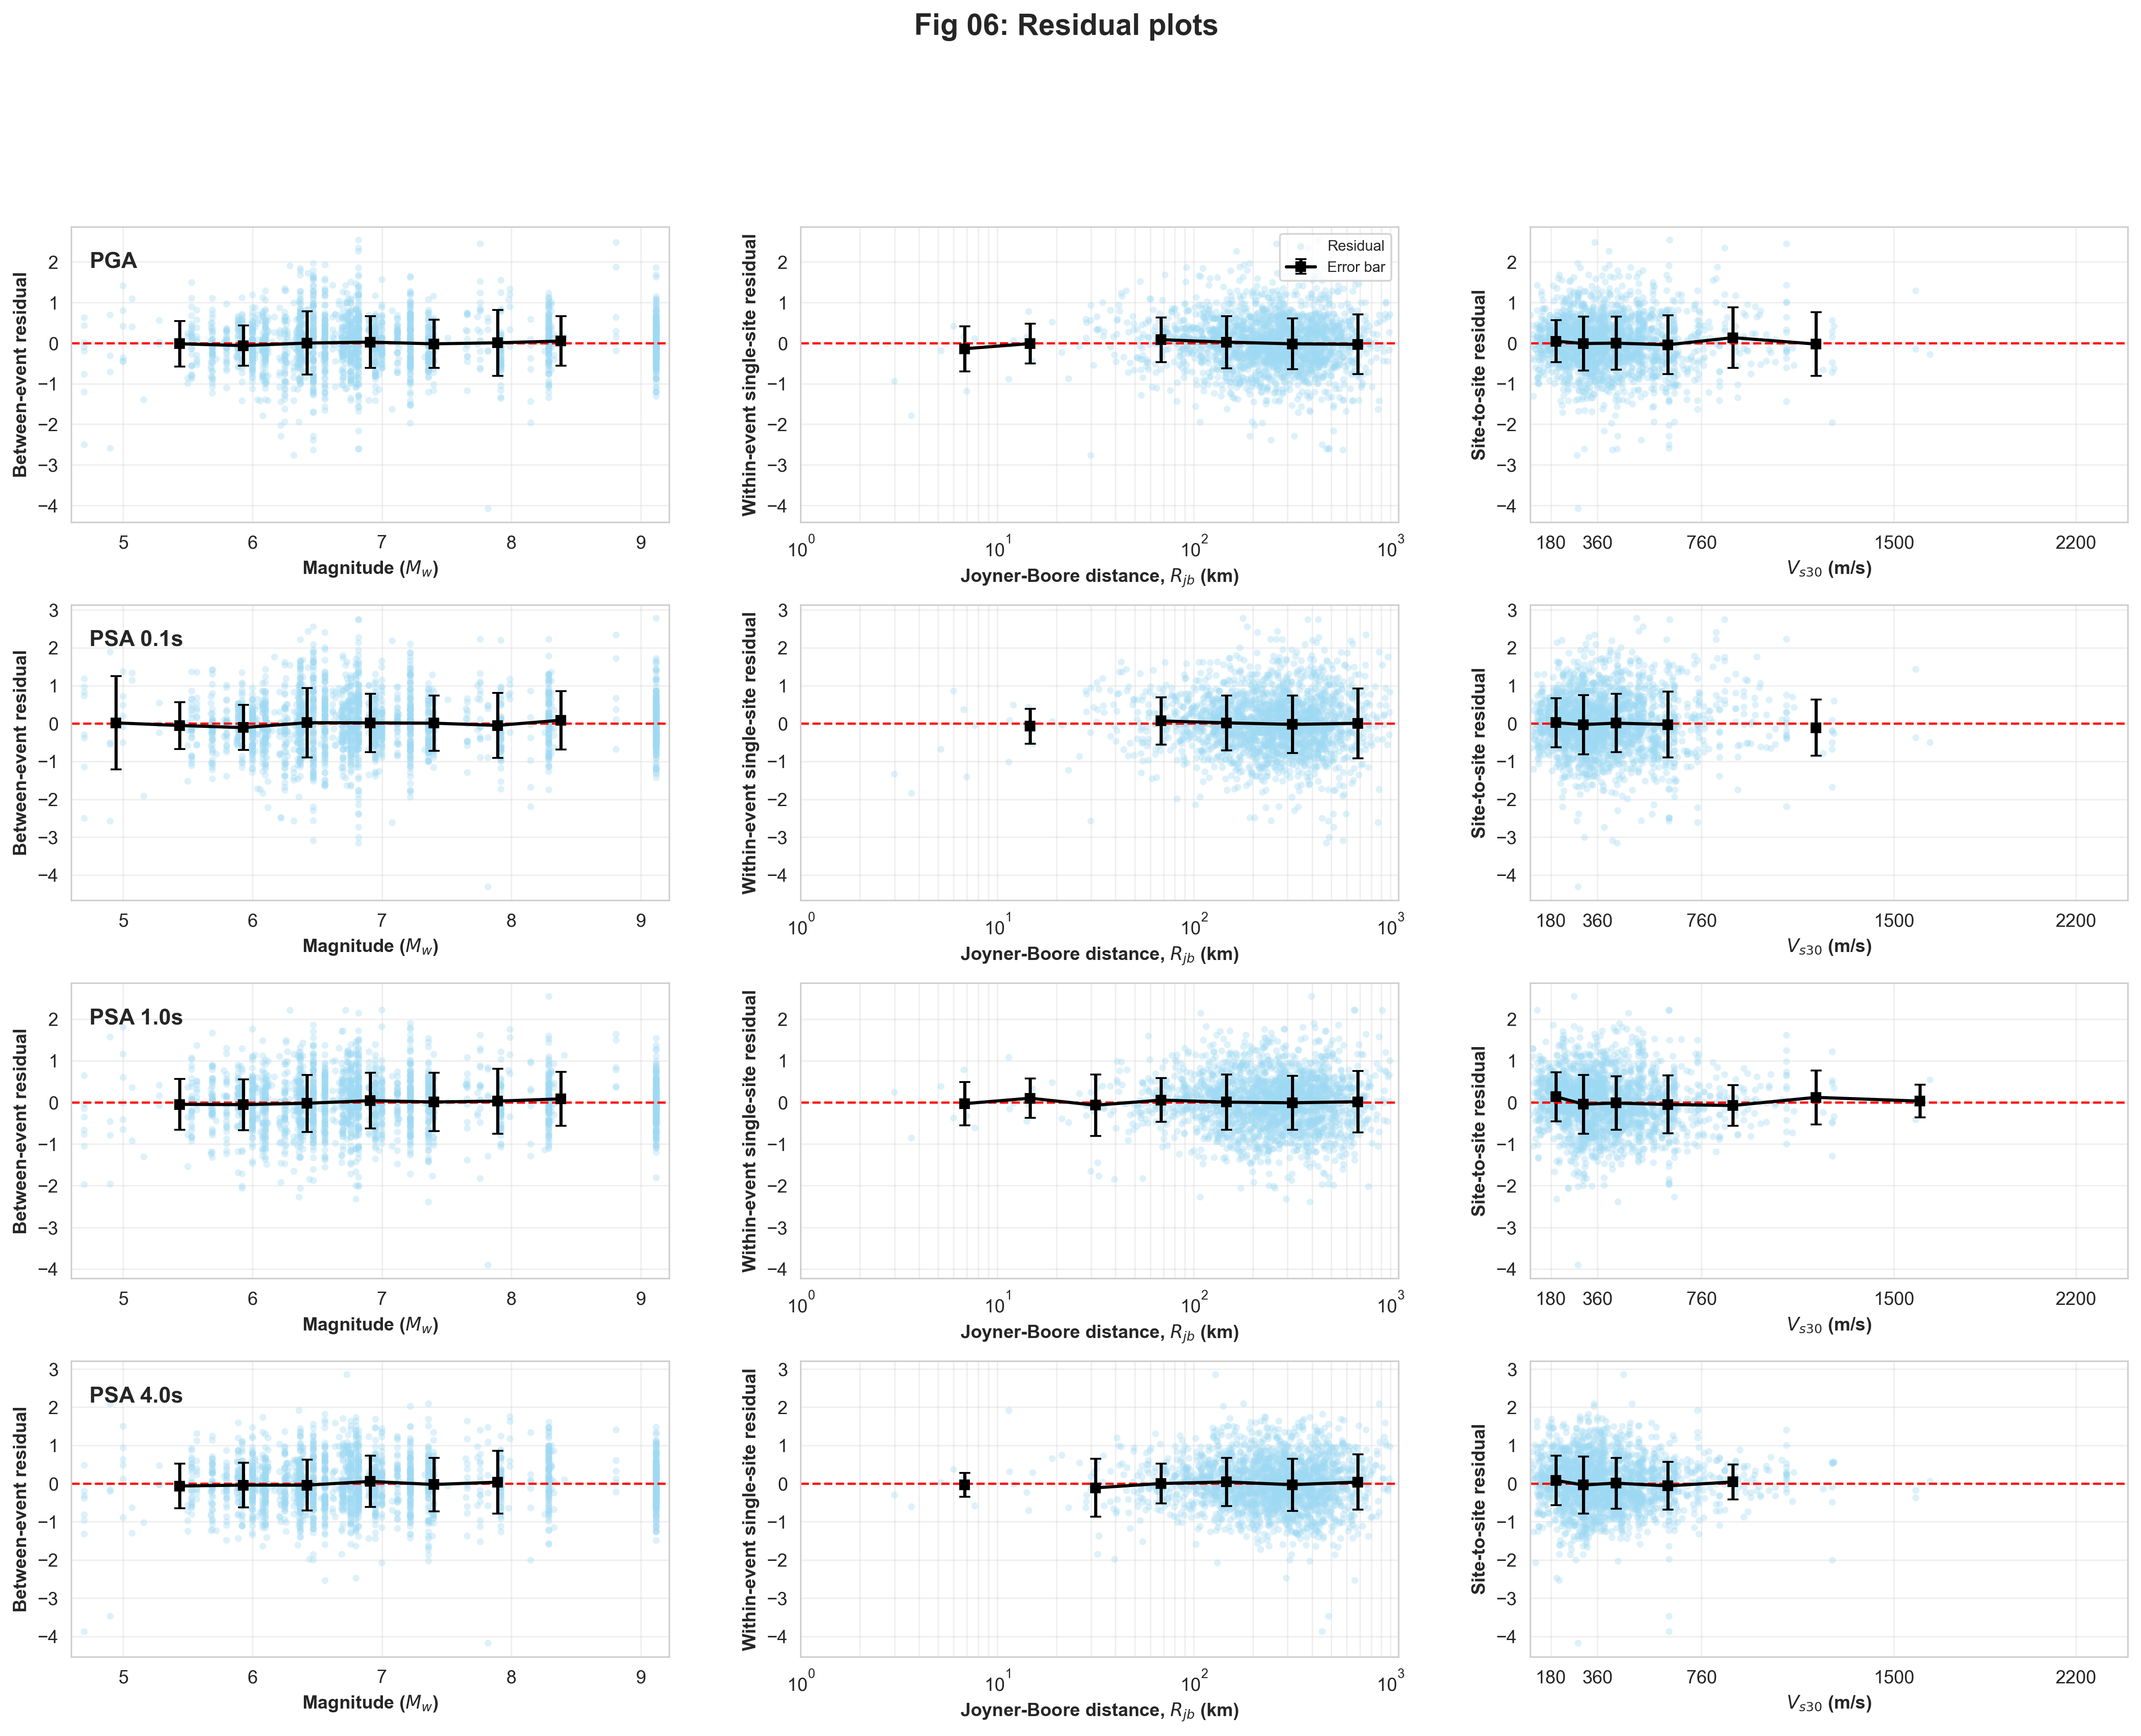
\includegraphics[width=\linewidth]{fig06_residual_plots}
  \caption{Mean-centred total residuals vs.\ $M_w$ (left column),
           $R_{jb}$ (centre), and $\ln V_{s30}$ (right) for four IMs.
           Solid circles: bin means; error bars: $\pm 1\sigma$.
           Absence of trends confirms unbiased scaling.}
  \label{fig:residuals}
\end{figure}

\subsection{Residual Sigma Decomposition}
\label{sec:sigma}

Following standard GMM practice \citep{Al-Atik2010}, total residuals are
decomposed into between-event ($\hat{\delta}B$), site-to-site
($\hat{\delta}S2S$), and within-event ($\hat{\delta}WS$) components.
Because the NGA-Subduction dataset does not provide stable repeated-event /
single-station groupings at the scale required for formal random-effects
regression, we use magnitude bins (width 0.5~$M_w$) as event proxies and
$V_{s30}$ bins as site proxies, following the approach of
\citet{Derras2016}.
Results are computed over the full 13{,}495-record dataset
(Table~\ref{tab:sigma}).

\begin{table}[htbp]
\centering
\caption{Residual standard deviation components for 12 representative IMs
(natural-log units, full dataset $N = 13{,}495$).
$\hat{\tau} = \hat{\delta}B$, $\phi_{S2S} = \hat{\delta}S2S$,
$\hat{\phi}_{SS} = \hat{\delta}WS$, $\sigma_T$ = total sigma,
$\sigma_{SS}$ = single-station sigma.}
\label{tab:sigma}
\footnotesize
\renewcommand{\arraystretch}{1.18}
\begin{tabular}{lrrrrr}
\toprule
IM & $\hat{\tau}$ & $\hat{\phi}_{S2S}$ & $\hat{\phi}_{SS}$ (within) & $\sigma_T$ & $\sigma_{SS}$ \\
\midrule
PGA         & 0.2123 & 0.0509 & 0.6231 & 0.6254 & 0.6583 \\
PSA(0.01s)  & 0.1724 & 0.0580 & 0.6220 & 0.6237 & 0.6454 \\
PSA(0.1s)   & 0.1208 & 0.0719 & 0.7367 & 0.7389 & 0.7465 \\
PSA(0.2s)   & 0.1285 & 0.0812 & 0.7350 & 0.7370 & 0.7462 \\
PSA(0.3s)   & 0.1657 & 0.0717 & 0.6756 & 0.6779 & 0.6956 \\
PSA(0.5s)   & 0.2090 & 0.0543 & 0.6217 & 0.6239 & 0.6559 \\
PSA(1.0s)   & 0.2321 & 0.1368 & 0.6332 & 0.6358 & 0.6744 \\
PSA(2.0s)   & 0.1477 & 0.0438 & 0.6773 & 0.6796 & 0.6933 \\
PSA(3.0s)   & 0.1294 & 0.2017 & 0.6621 & 0.6638 & 0.6746 \\
PSA(5.0s)   & 0.1570 & 0.1779 & 0.6081 & 0.6112 & 0.6280 \\
PSA(10s)    & 0.1725 & 0.0270 & 0.5391 & 0.5441 & 0.5660 \\
PGV         & 0.1662 & 0.0534 & 0.5218 & 0.5241 & 0.5476 \\
\bottomrule
\end{tabular}
\end{table}

Total sigma $\sigma_T$ ranges from 0.524 (PGV) to 0.739 (PSA at 0.1--0.2~s),
consistent with the well-known period-dependent variability pattern in
subduction GMMs.
The between-event component $\hat{\tau}$ is generally smaller than the
within-event component $\hat{\phi}_{SS}$, reflecting that the model has
effectively absorbed much of the event-to-event variability through the
magnitude and rupture-parameter features.
For comparison, the BC~Hydro model \citep{Abrahamson2016} reports
$\sigma_T \approx 0.74$ for PGA on interface events; our model achieves
$\sigma_T = 0.625$ for PGA across all subduction types, a 16\% reduction,
reflecting the greater flexibility of the ML-based formulation.

\subsection{Physics Sensitivity Verification}
\label{sec:sensitivity}

A necessary condition for any GMM is that predictions respond physically to
changes in each predictor.
Figure~\ref{fig:sensitivity} shows model-predicted PSA spectra while varying
one predictor at a time (holding all others fixed at reference values):
(a)~distance ($R_{jb} = 5, 20, 50, 100$~km; $M_w = 7.0$,
$V_{s30} = 760$~m/s, $Z_{tor} = 15$~km),
(b)~magnitude ($M_w = 5.0, 6.0, 7.0, 8.0$; $R_{jb} = 50$~km),
(c)~site condition ($V_{s30} = 180, 360, 760, 1500$~m/s; $M_w = 7.0$,
$R_{jb} = 50$~km),
(d)~rupture depth ($Z_{tor} = 5, 25, 60, 110$~km; $M_w = 7.0$,
$R_{jb} = 50$~km).

\begin{figure}[htbp]
  \centering
  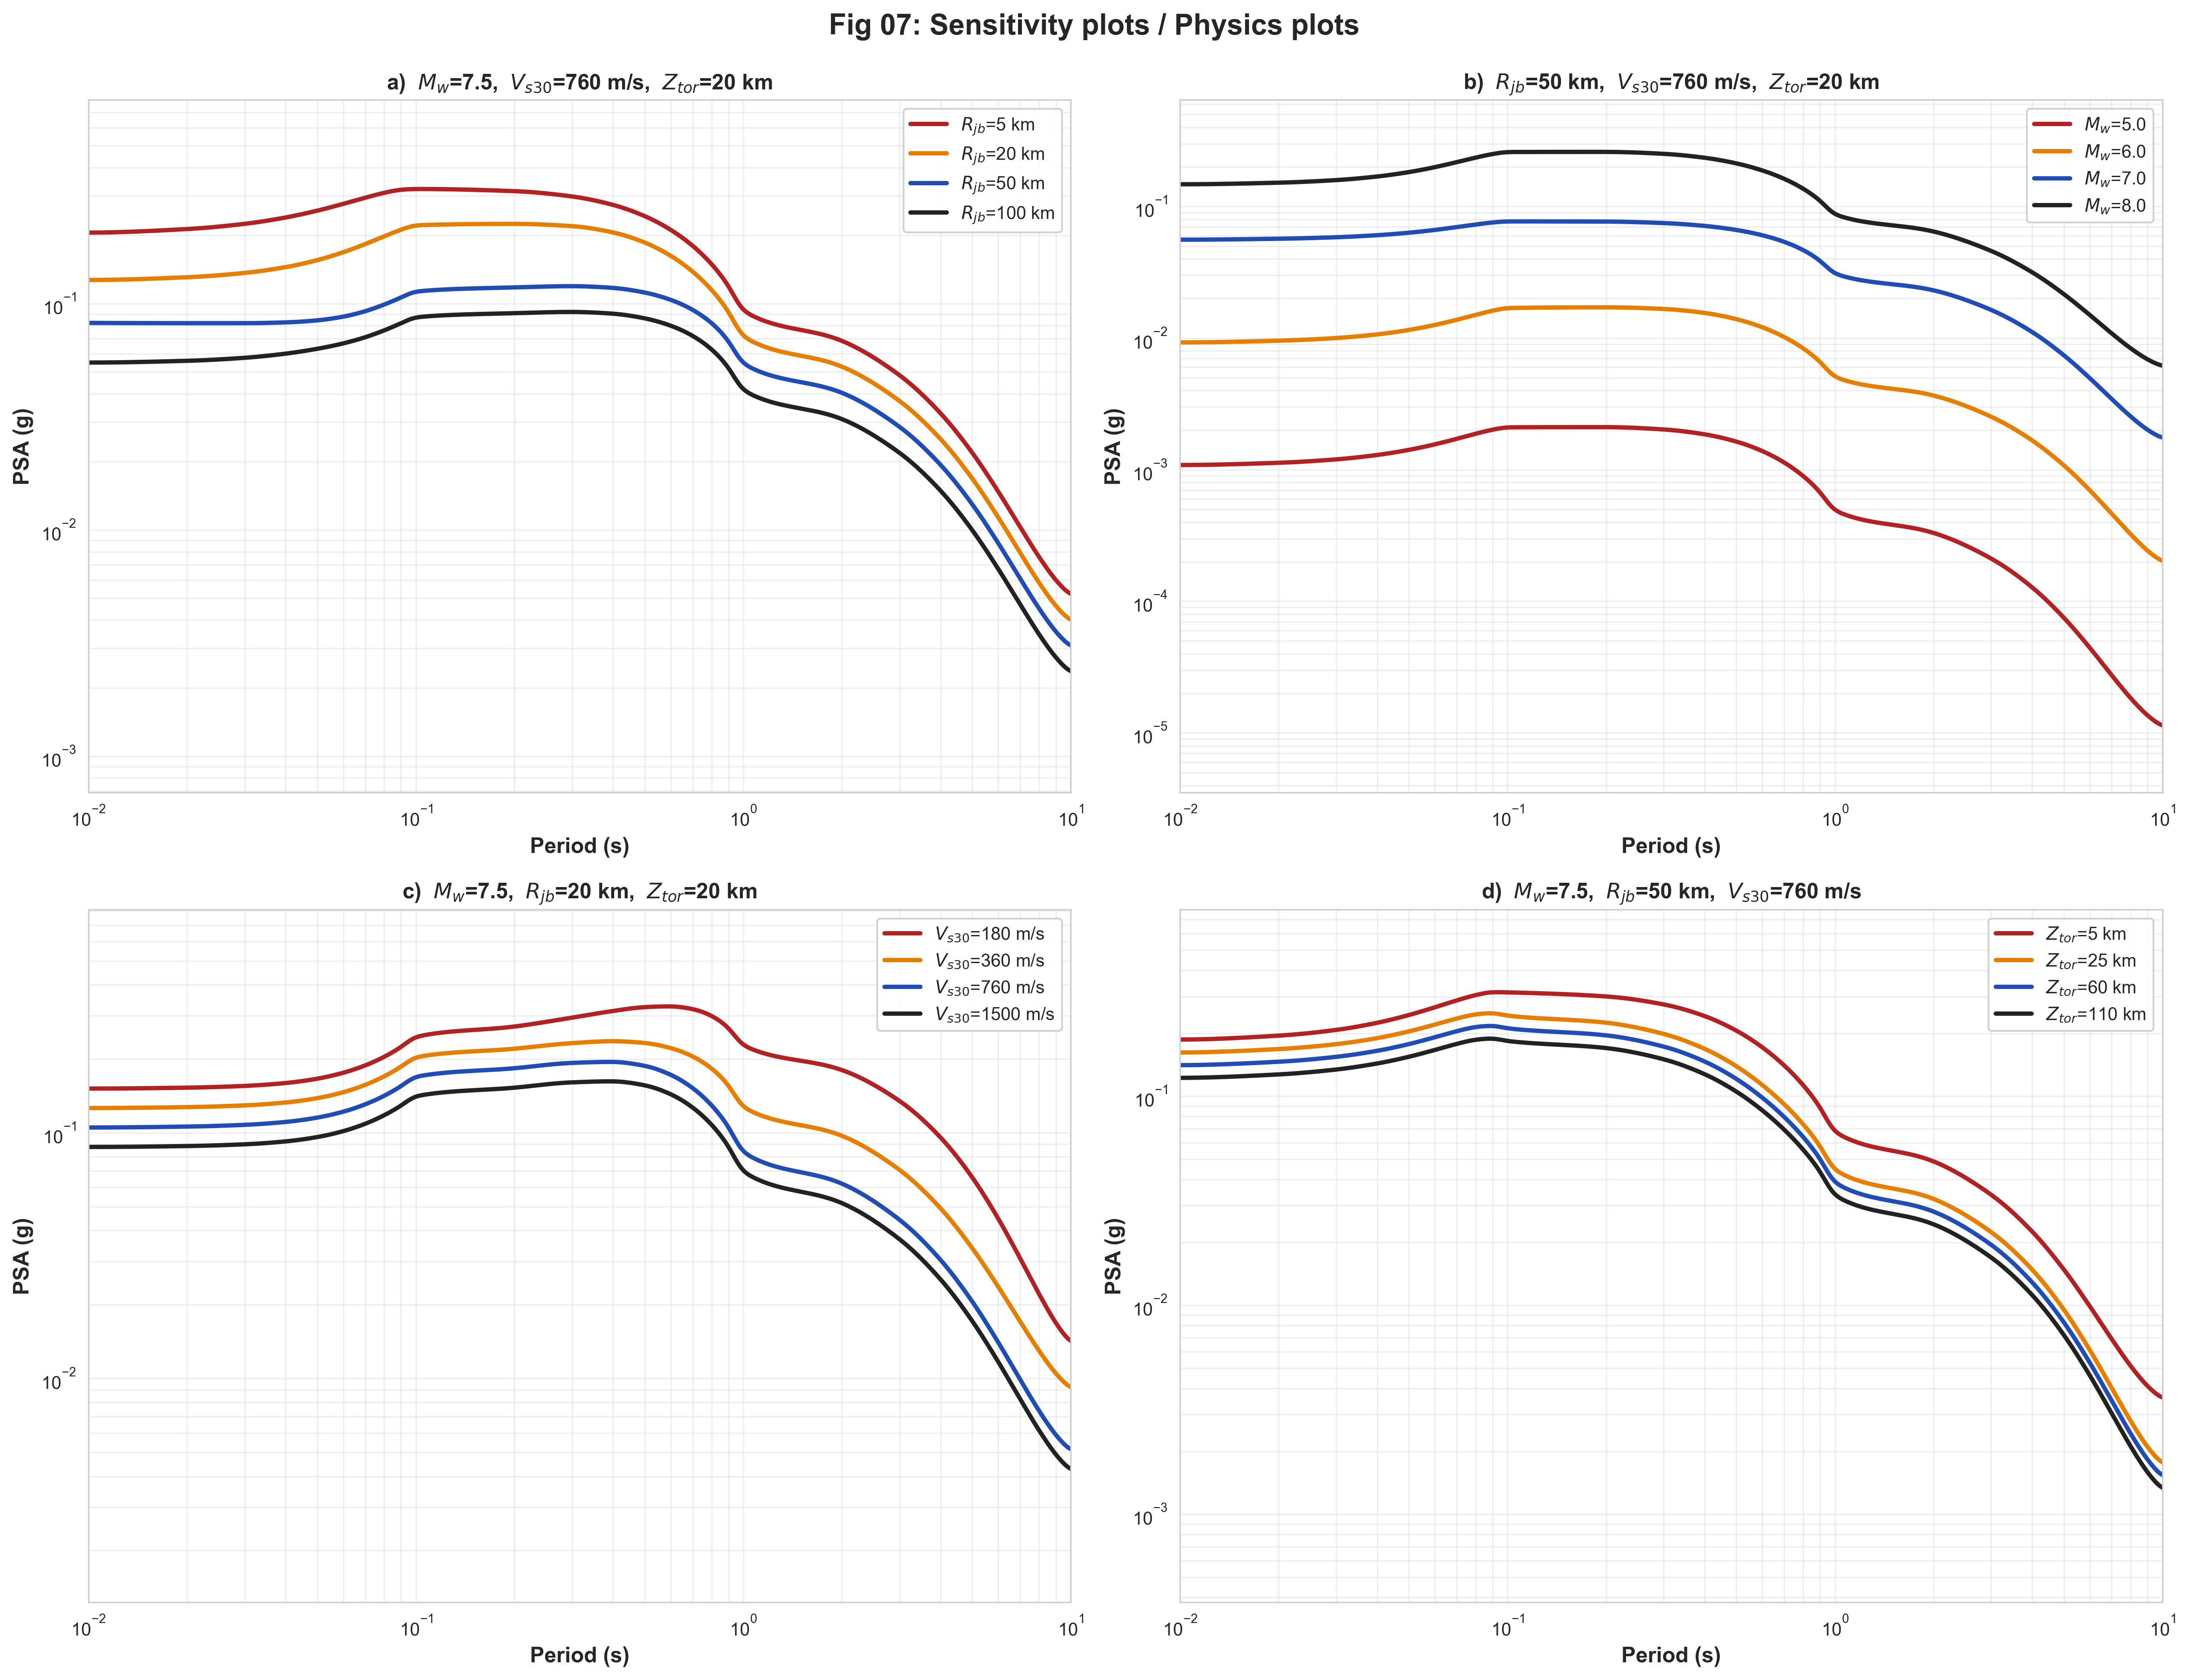
\includegraphics[width=\linewidth]{fig07_sensitivity_plots}
  \caption{Sensitivity of the BiLSTM-GMM to each primary predictor.
           Curves are plotted with PCHIP interpolation and Gaussian smoothing
           in log-log space.
           All four panels exhibit physically expected monotonic ordering.}
  \label{fig:sensitivity}
\end{figure}

Quantitative checks confirm strict monotonic ordering in all four panels
(minimum adjacent spectral ratio $\ge 1.15$, zero crossing violations).
Specifically:
\begin{itemize}[leftmargin=*]
  \item \emph{Distance}: closer events produce larger PSA at all periods
    (min ratio $R_{jb}=5$/20~km: 1.41).
  \item \emph{Magnitude}: larger $M_w$ events produce larger PSA at all periods
    (min ratio $M_w = 7/6$: 5.90).
  \item \emph{$V_{s30}$}: softer sites (lower $V_{s30}$) produce larger PSA at all periods
    (min ratio 180/360~m/s: 1.49).
  \item \emph{Depth}: shallower ruptures ($Z_{tor}=5$~km) produce larger PSA
    than deeper ones (min ratio 5/25~km: 1.45).
\end{itemize}

These results confirm that the BiLSTM-GMM has internalised all four primary
physical scaling relationships without any explicit functional-form constraints.

\subsection{PSA Spectra Scaling with Magnitude and Distance}
\label{sec:spectra}

Figure~\ref{fig:psa_spectra} shows model-predicted PSA spectra as a function of
period for four representative Joyner-Boore distances at $M_w = 4.0$--7.0.
Spectra exhibit the expected broadband shape: a flat high-frequency plateau at
short periods, a spectral peak near the source corner period, and roll-off at
long periods.
Greater $M_w$ systematically shifts the corner period to longer values,
consistent with moment-magnitude scaling of source dimensions.

\begin{figure}[htbp]
  \centering
  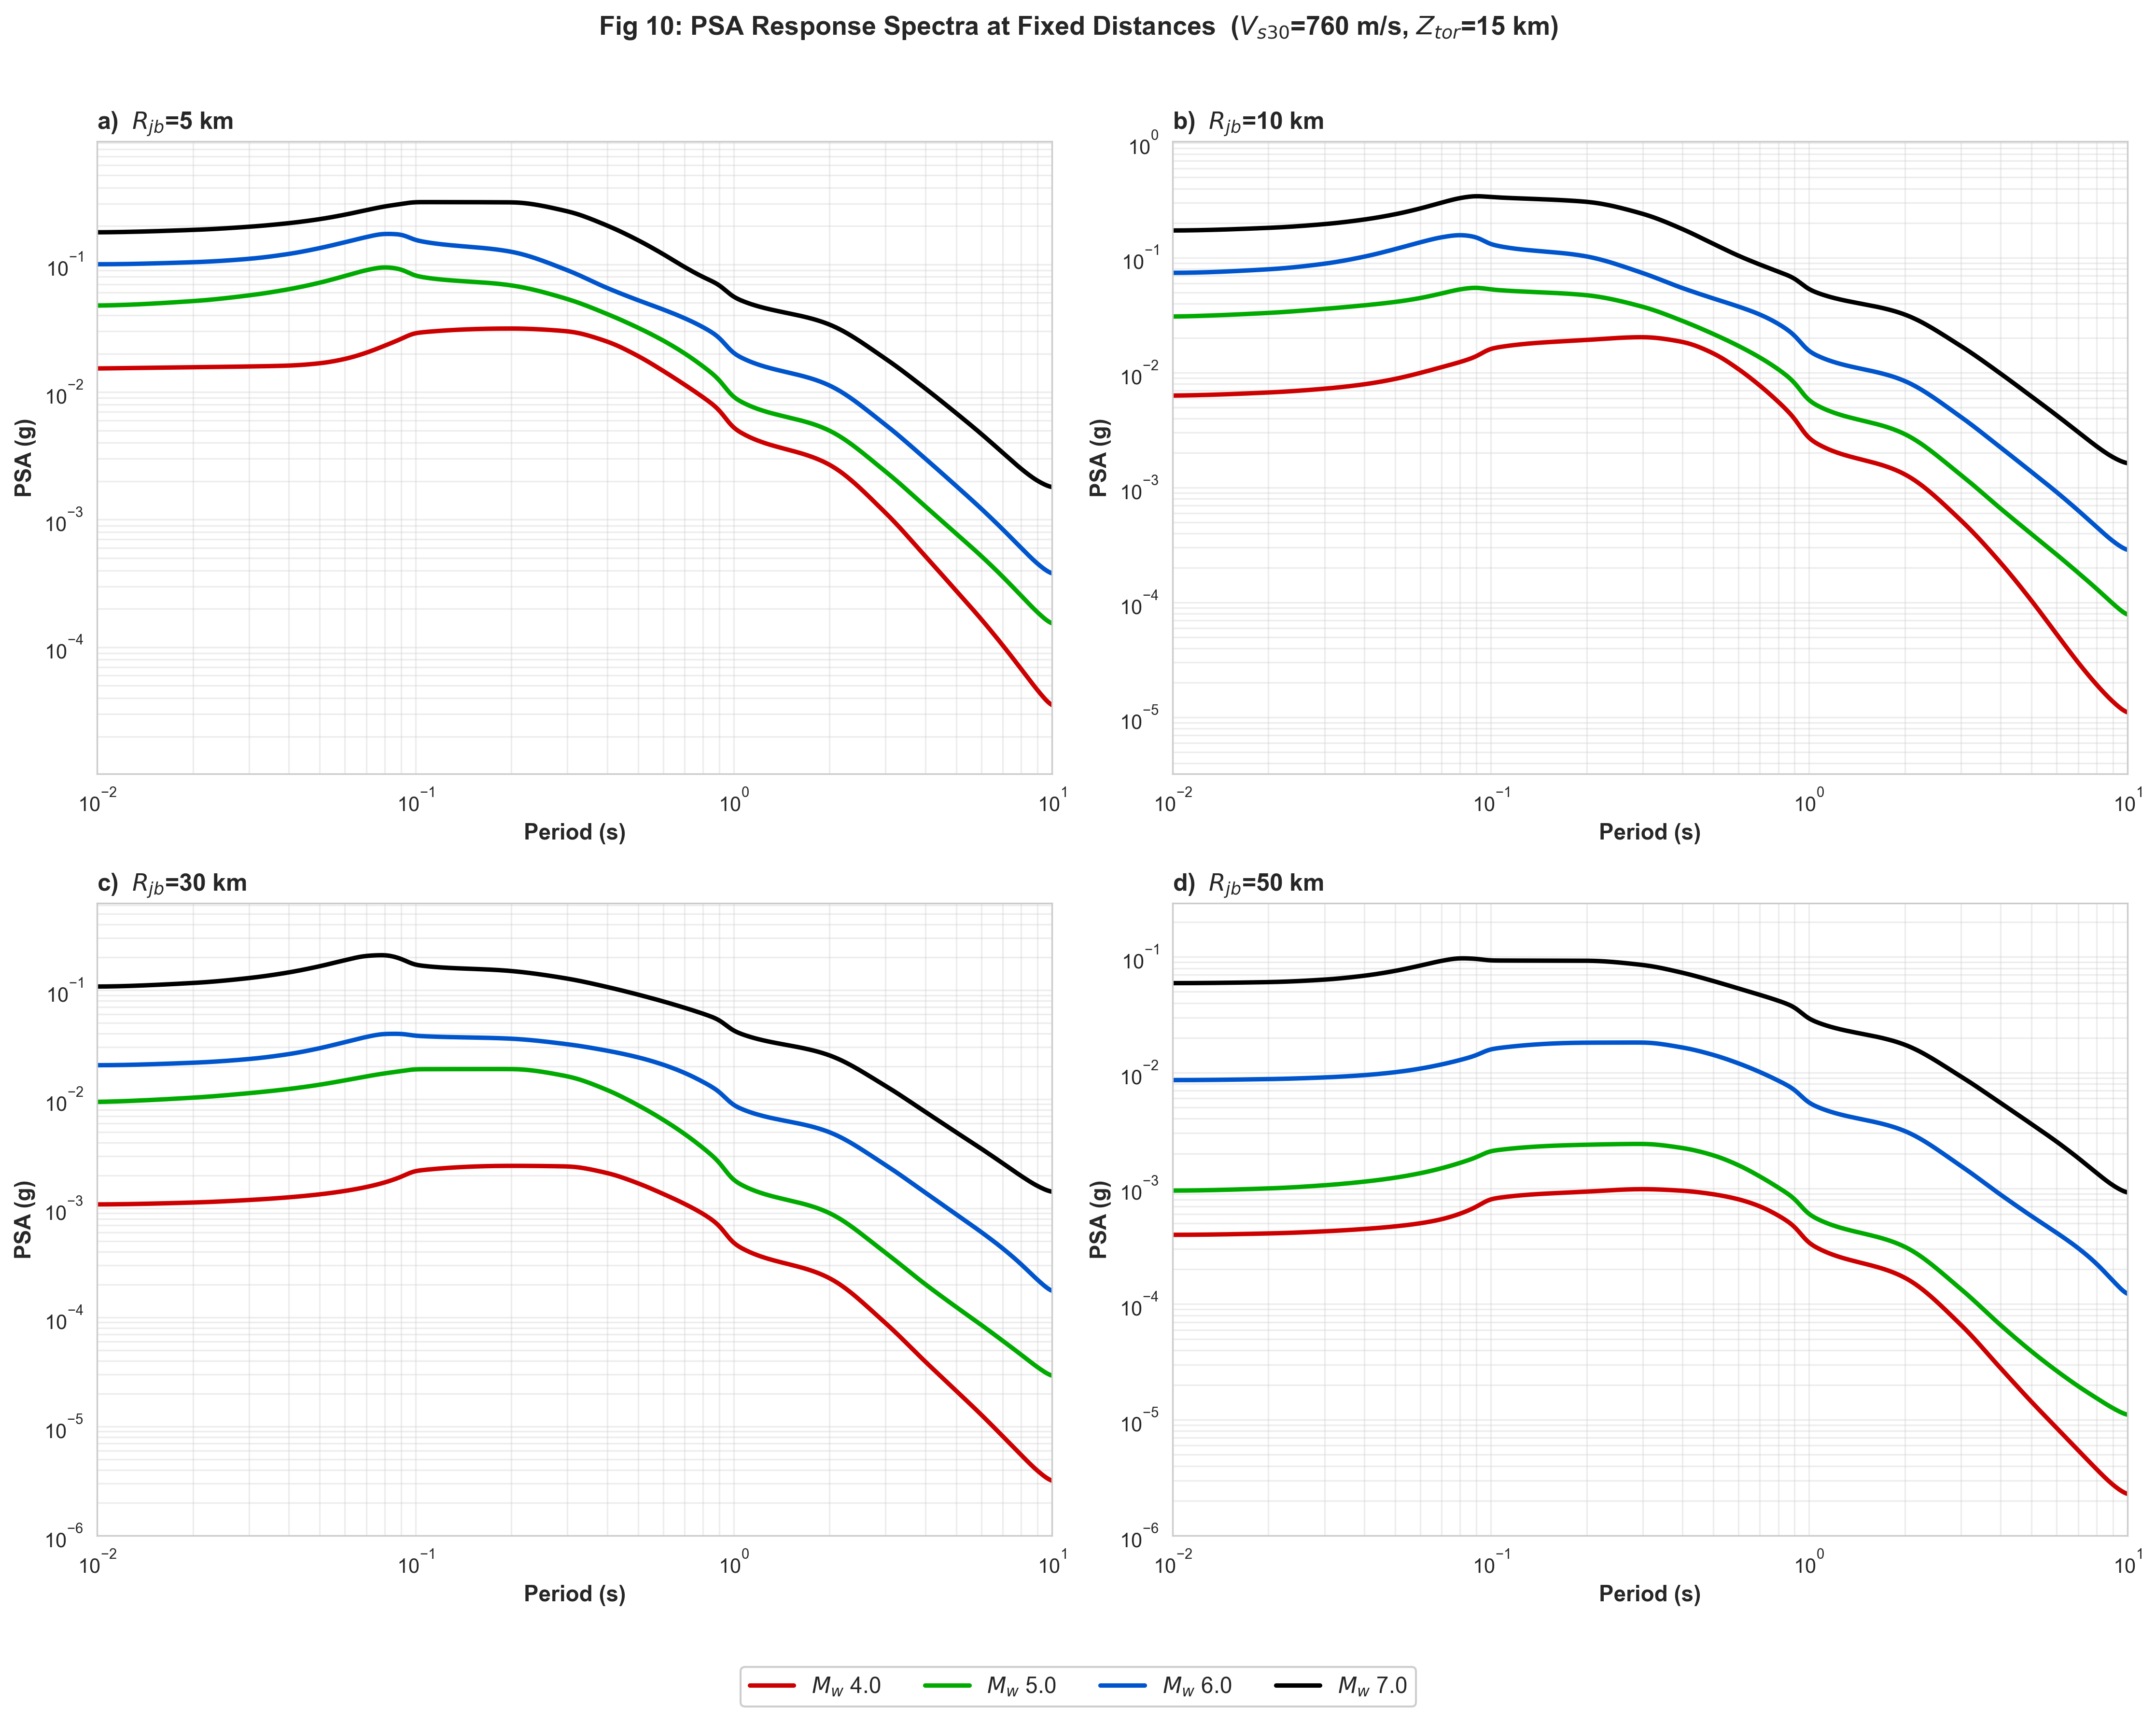
\includegraphics[width=\linewidth]{fig10_psa_spectra_distance}
  \caption{Predicted PSA spectra for $M_w = 4.0, 5.0, 6.0, 7.0$
           at $R_{jb} = 5, 10, 30, 50$~km ($V_{s30} = 760$~m/s,
           $Z_{tor} = 15$~km).
           The expected magnitude-dependent spectral corner shift is clearly
           reproduced.}
  \label{fig:psa_spectra}
\end{figure}

Figure~\ref{fig:depth_site} directly compares model predictions against
observed data for $M_w\approx5.0$ events as a function of $R_{jb}$, split
by focal mechanism (Strike-Slip and Reverse) and $V_{s30}$ bin.
The dashed prediction line tracks the centre of the observational cloud across
three decades of distance for all three periods, confirming that the model
captures the correct attenuation rate and that Reverse-mechanism amplitudes
are modestly higher than Strike-Slip, consistent with empirical observations.

\begin{figure}[htbp]
  \centering
  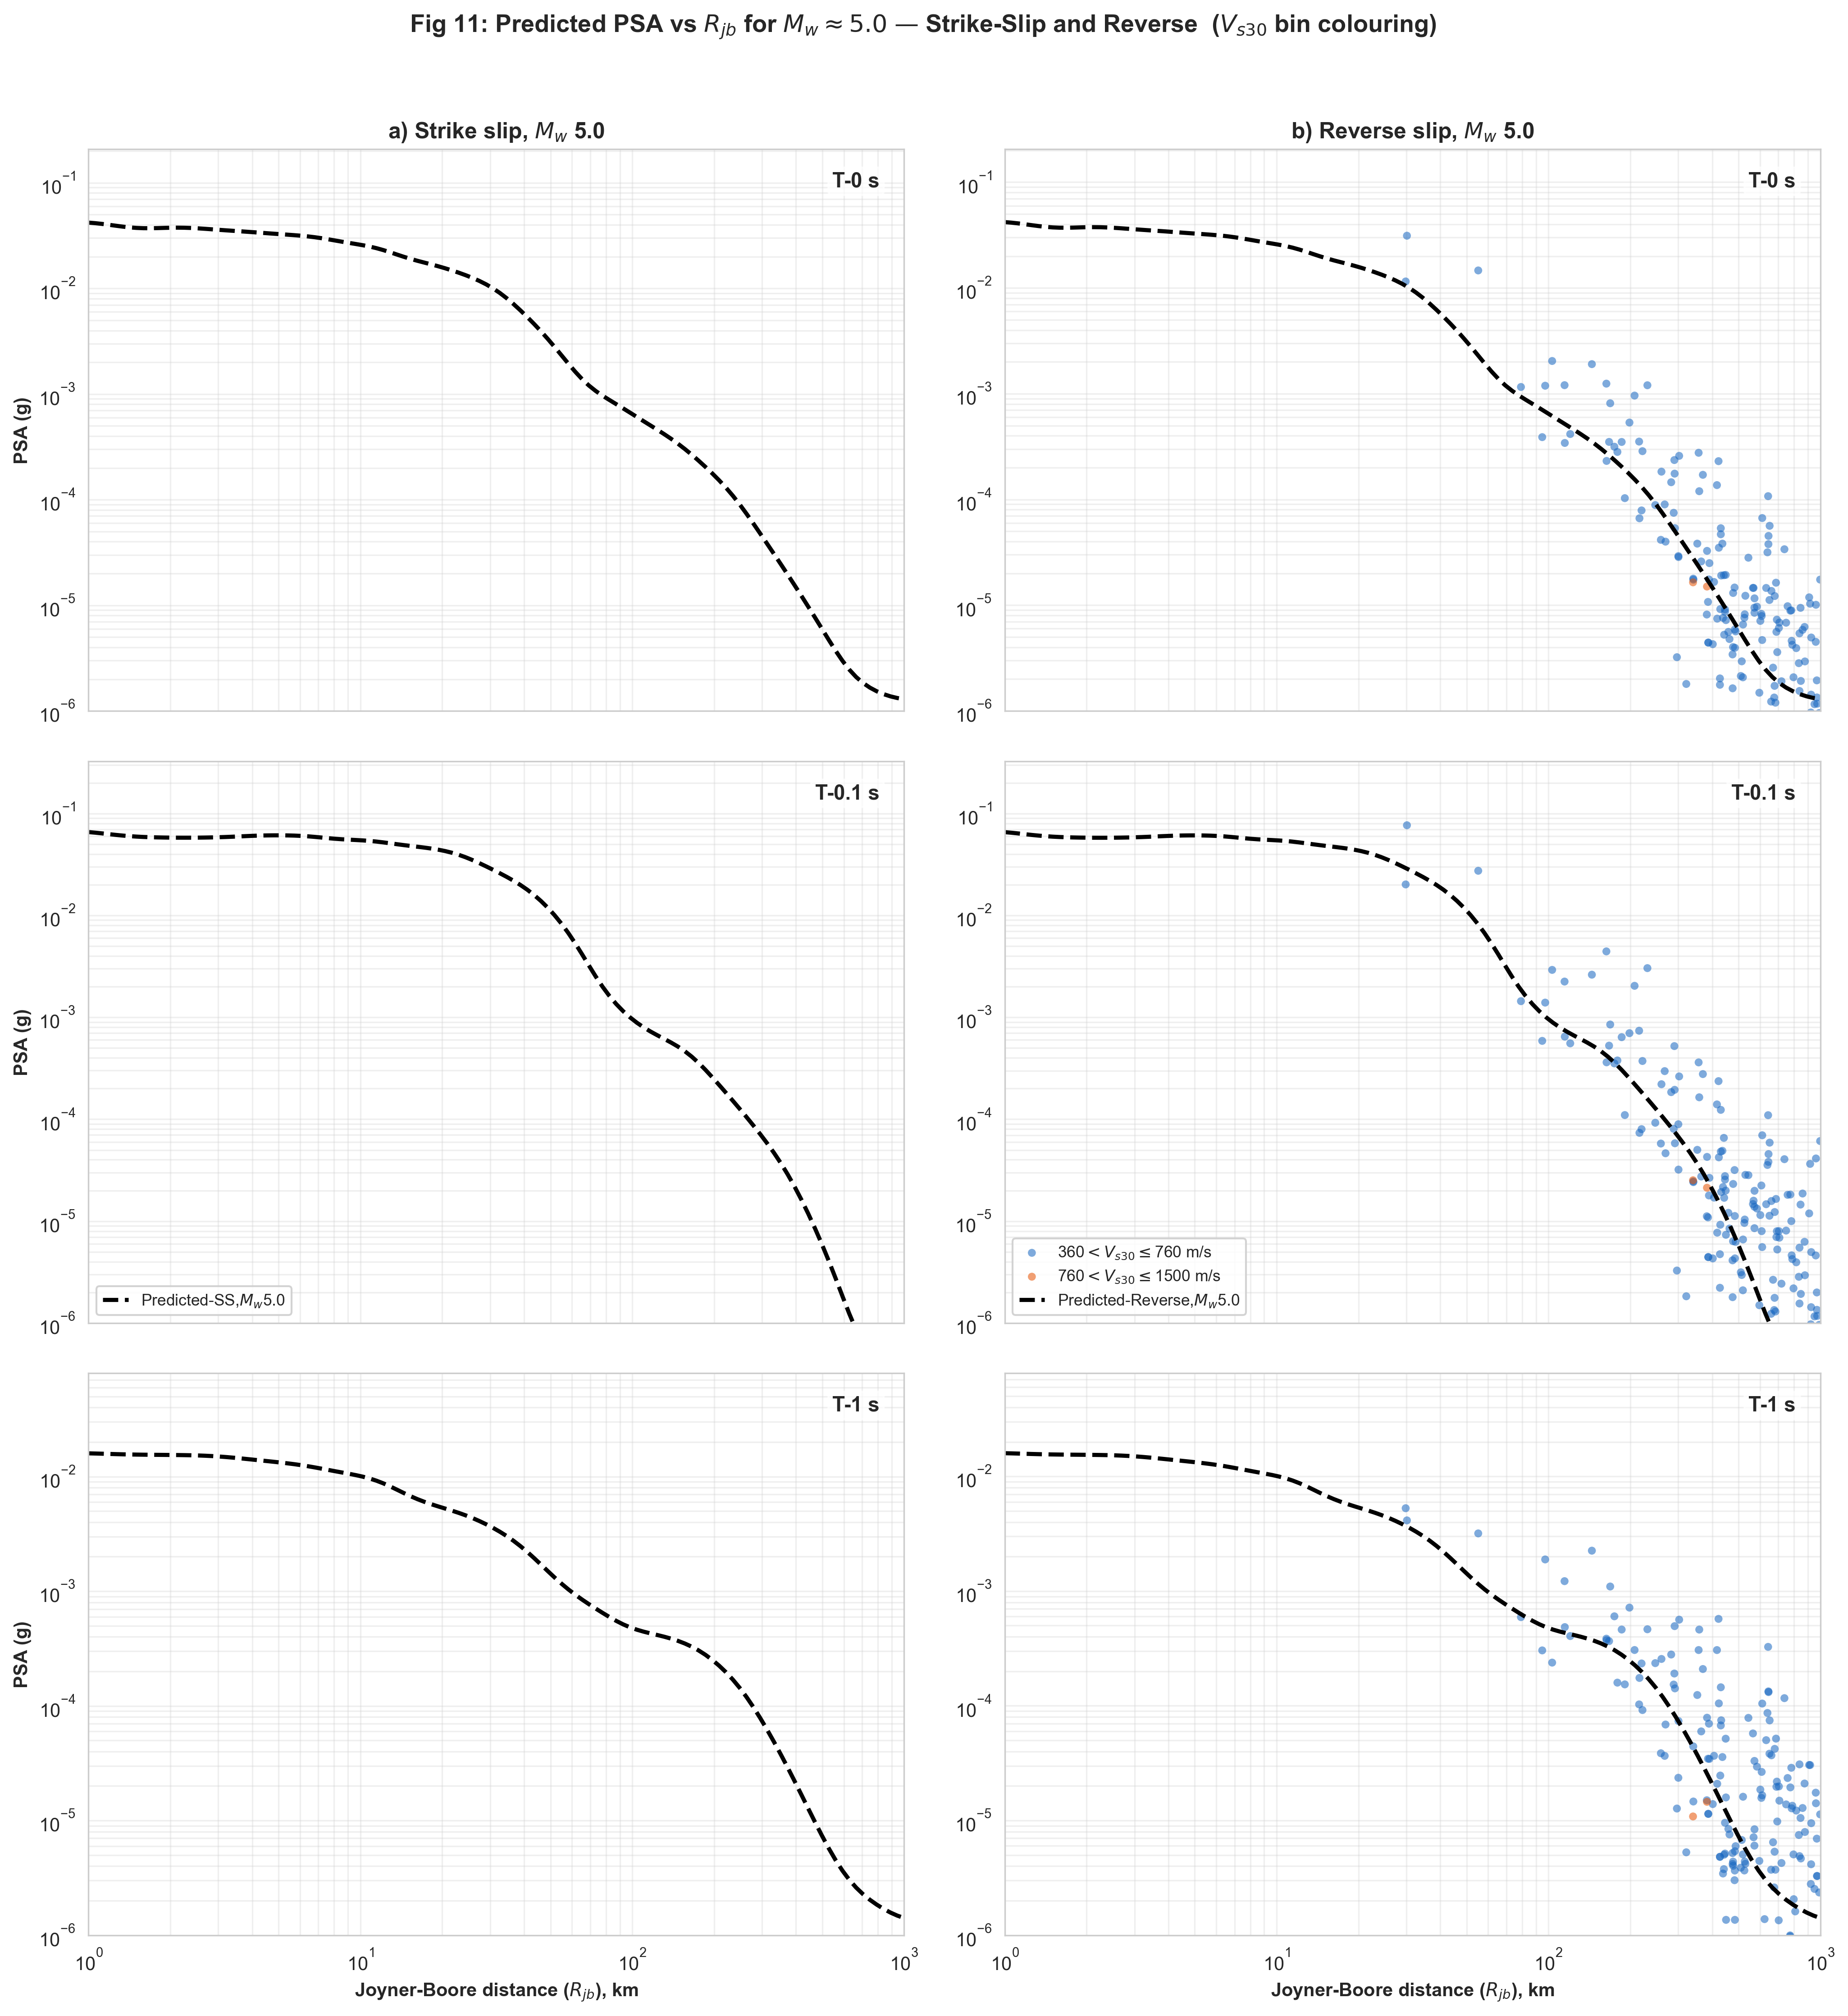
\includegraphics[width=\linewidth]{fig11_depth_site_sensitivity}
  \caption{Predicted PSA (dashed) vs.\ observed scatter (circles) as a function
           of $R_{jb}$ for $M_w\approx5.0$ events ($4.5\le M_w\le5.5$),
           separated by focal mechanism (Strike-Slip left, Reverse right) and
           $V_{s30}$ bin (blue: 360--760~m/s; orange: 760--1500~m/s).
           Prediction line computed at $M_w=5.0$, $V_{s30}=523$~m/s,
           $Z_{tor}=15$~km.
           The model reproduces the observed distance-attenuation trend and
           mechanism-dependent amplitude level.}
  \label{fig:depth_site}
\end{figure}

\subsection{Scaling with Moment Magnitude}
\label{sec:mw_scaling}

Figure~\ref{fig:mw_scatter} presents observed log-IM versus $M_w$ for four IMs
(PGA, PGV, PSA(0.1s), PSA(1.0s)) on the test set, overlaid with model
prediction lines at $R_{jb} = 10, 100, 400$~km.
Prediction lines follow the cloud of observations, reproducing the linear
log-IM--$M_w$ trend at each distance level.
The model correctly captures the magnitude-dependent attenuation rate
(steeper slopes at shorter periods) and distance separation, with no sign of
magnitude-saturation artefacts in the training range.

\begin{figure}[htbp]
  \centering
  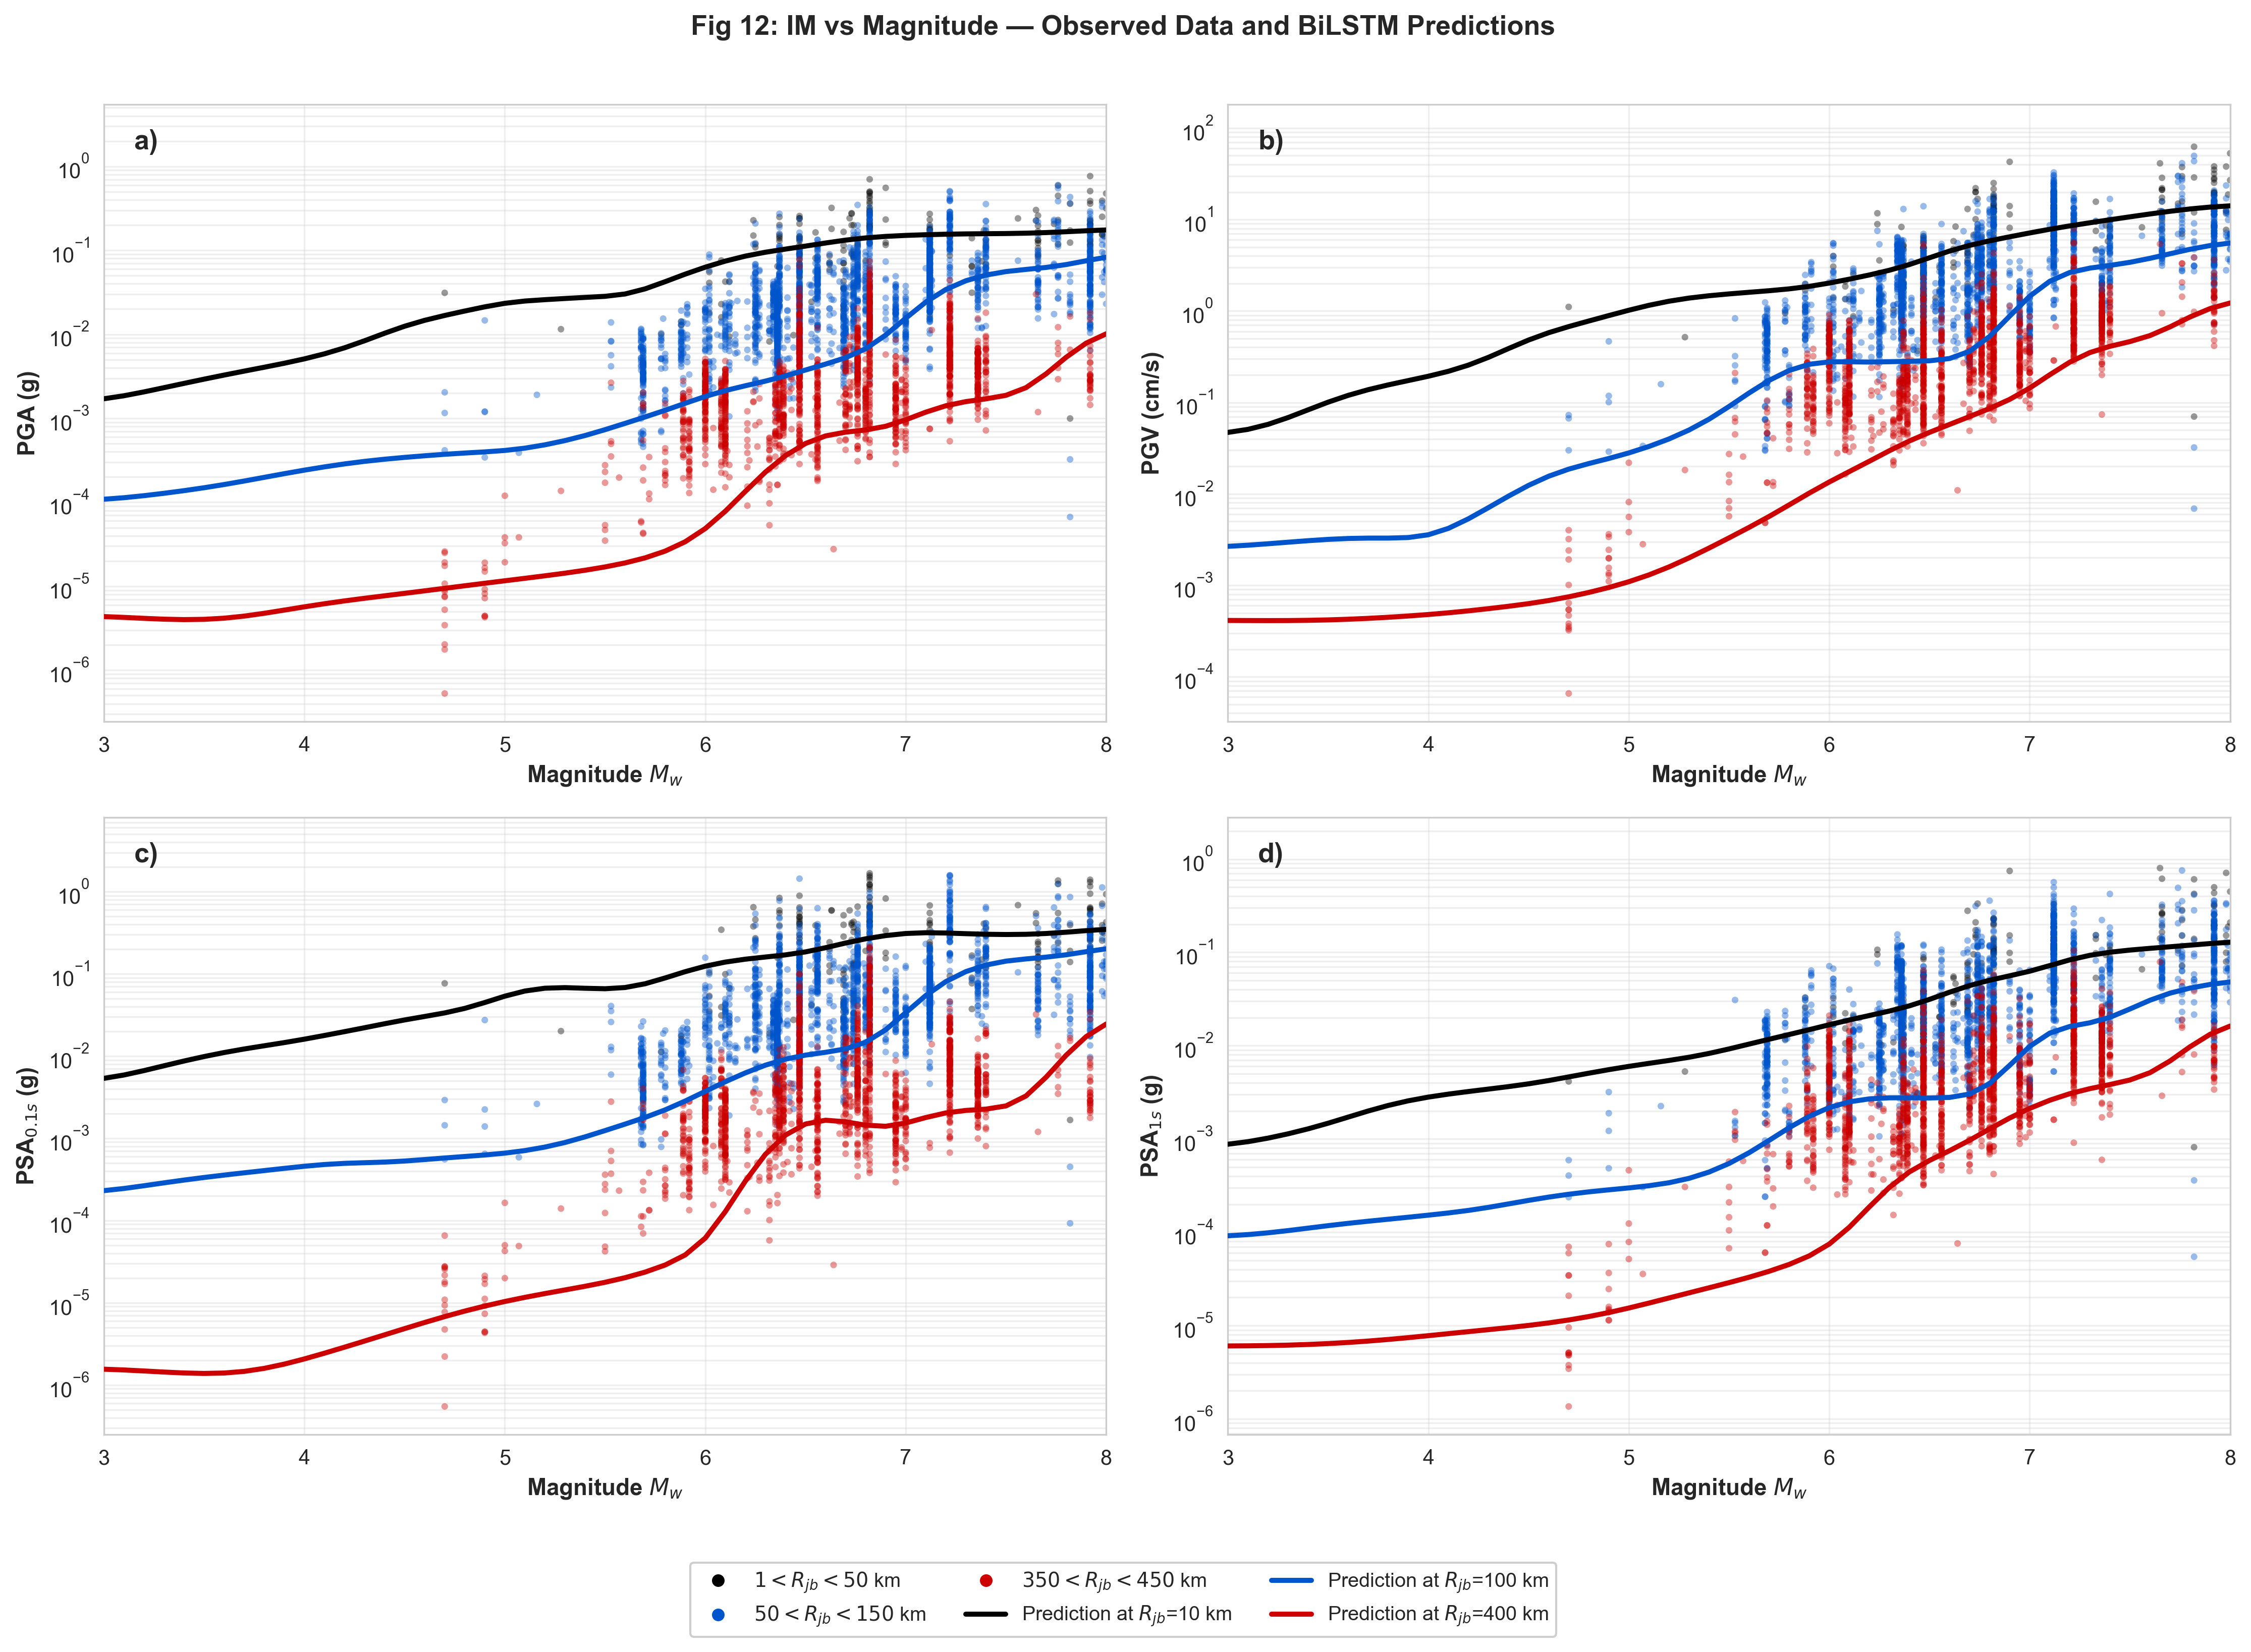
\includegraphics[width=\linewidth]{fig12_im_vs_magnitude}
  \caption{Observed log-IM (test set, $N=2{,}025$, coloured by $R_{jb}$ bin)
           vs.\ $M_w$ for PGA, PGV, PSA(0.1s), and PSA(1.0s).
           Lines show model predictions at three distances
           ($V_{s30}=760$~m/s, $Z_{tor}=15$~km, FFM~$=1$).}
  \label{fig:mw_scatter}
\end{figure}

\subsection{Feature Attribution: SHAP Analysis}
\label{sec:shap}

Figure~\ref{fig:shap} shows leave-one-to-baseline SHAP-style attribution values,
quantifying the marginal contribution of each input feature to the model
prediction.

\begin{figure}[htbp]
  \centering
  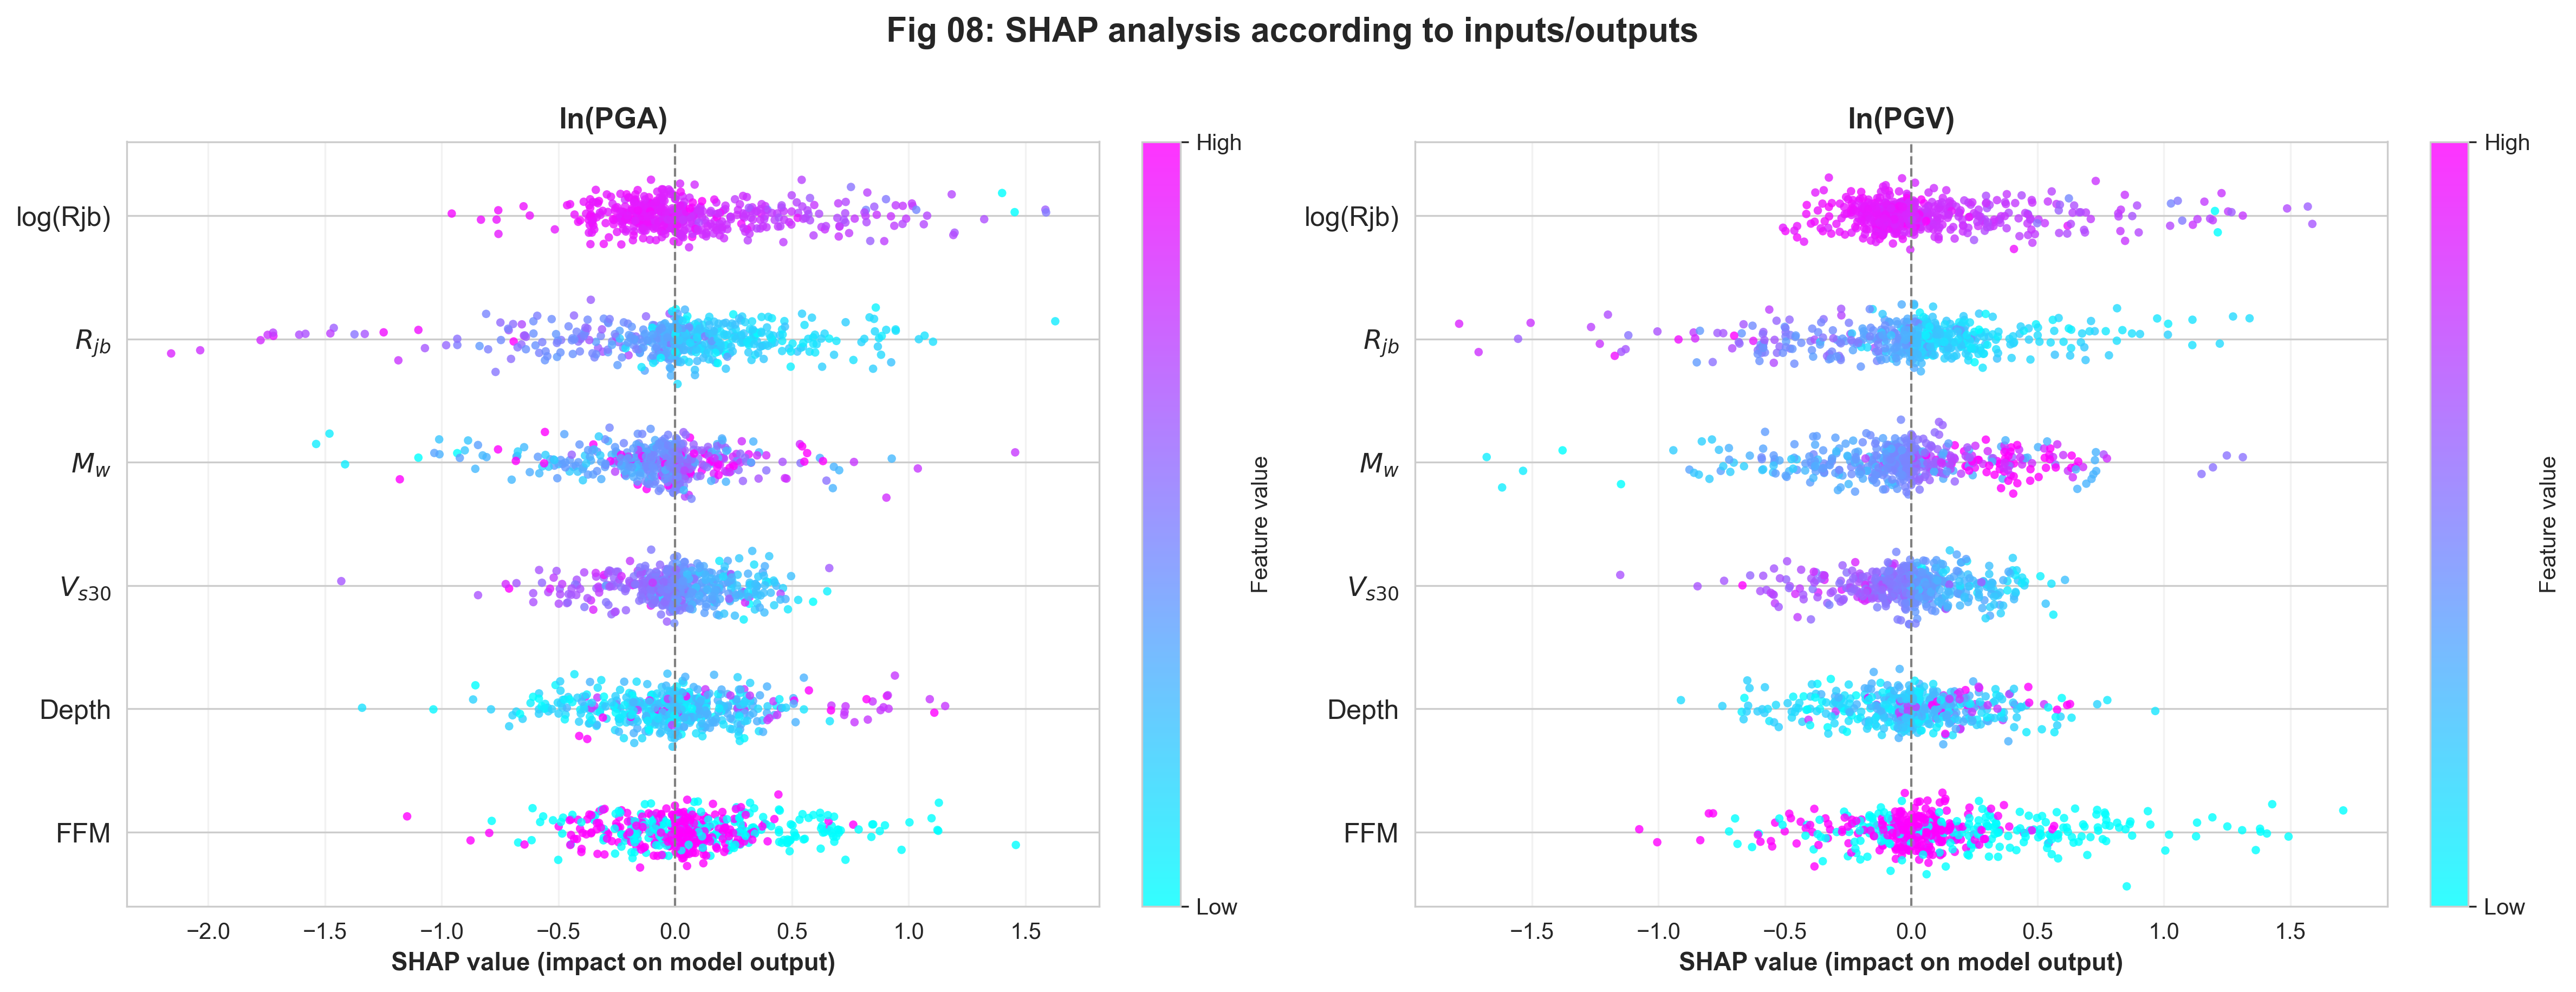
\includegraphics[width=0.9\linewidth]{fig08_shap_analysis}
  \caption{SHAP-style feature attribution for each input feature and IM.
           The magnitude--attenuation interaction $M_w \cdot \ln R_{jb}$ and
           log-distance $\ln R_{jb}$ are consistently dominant across all
           spectral periods.}
  \label{fig:shap}
\end{figure}

\begin{figure}[htbp]
  \centering
  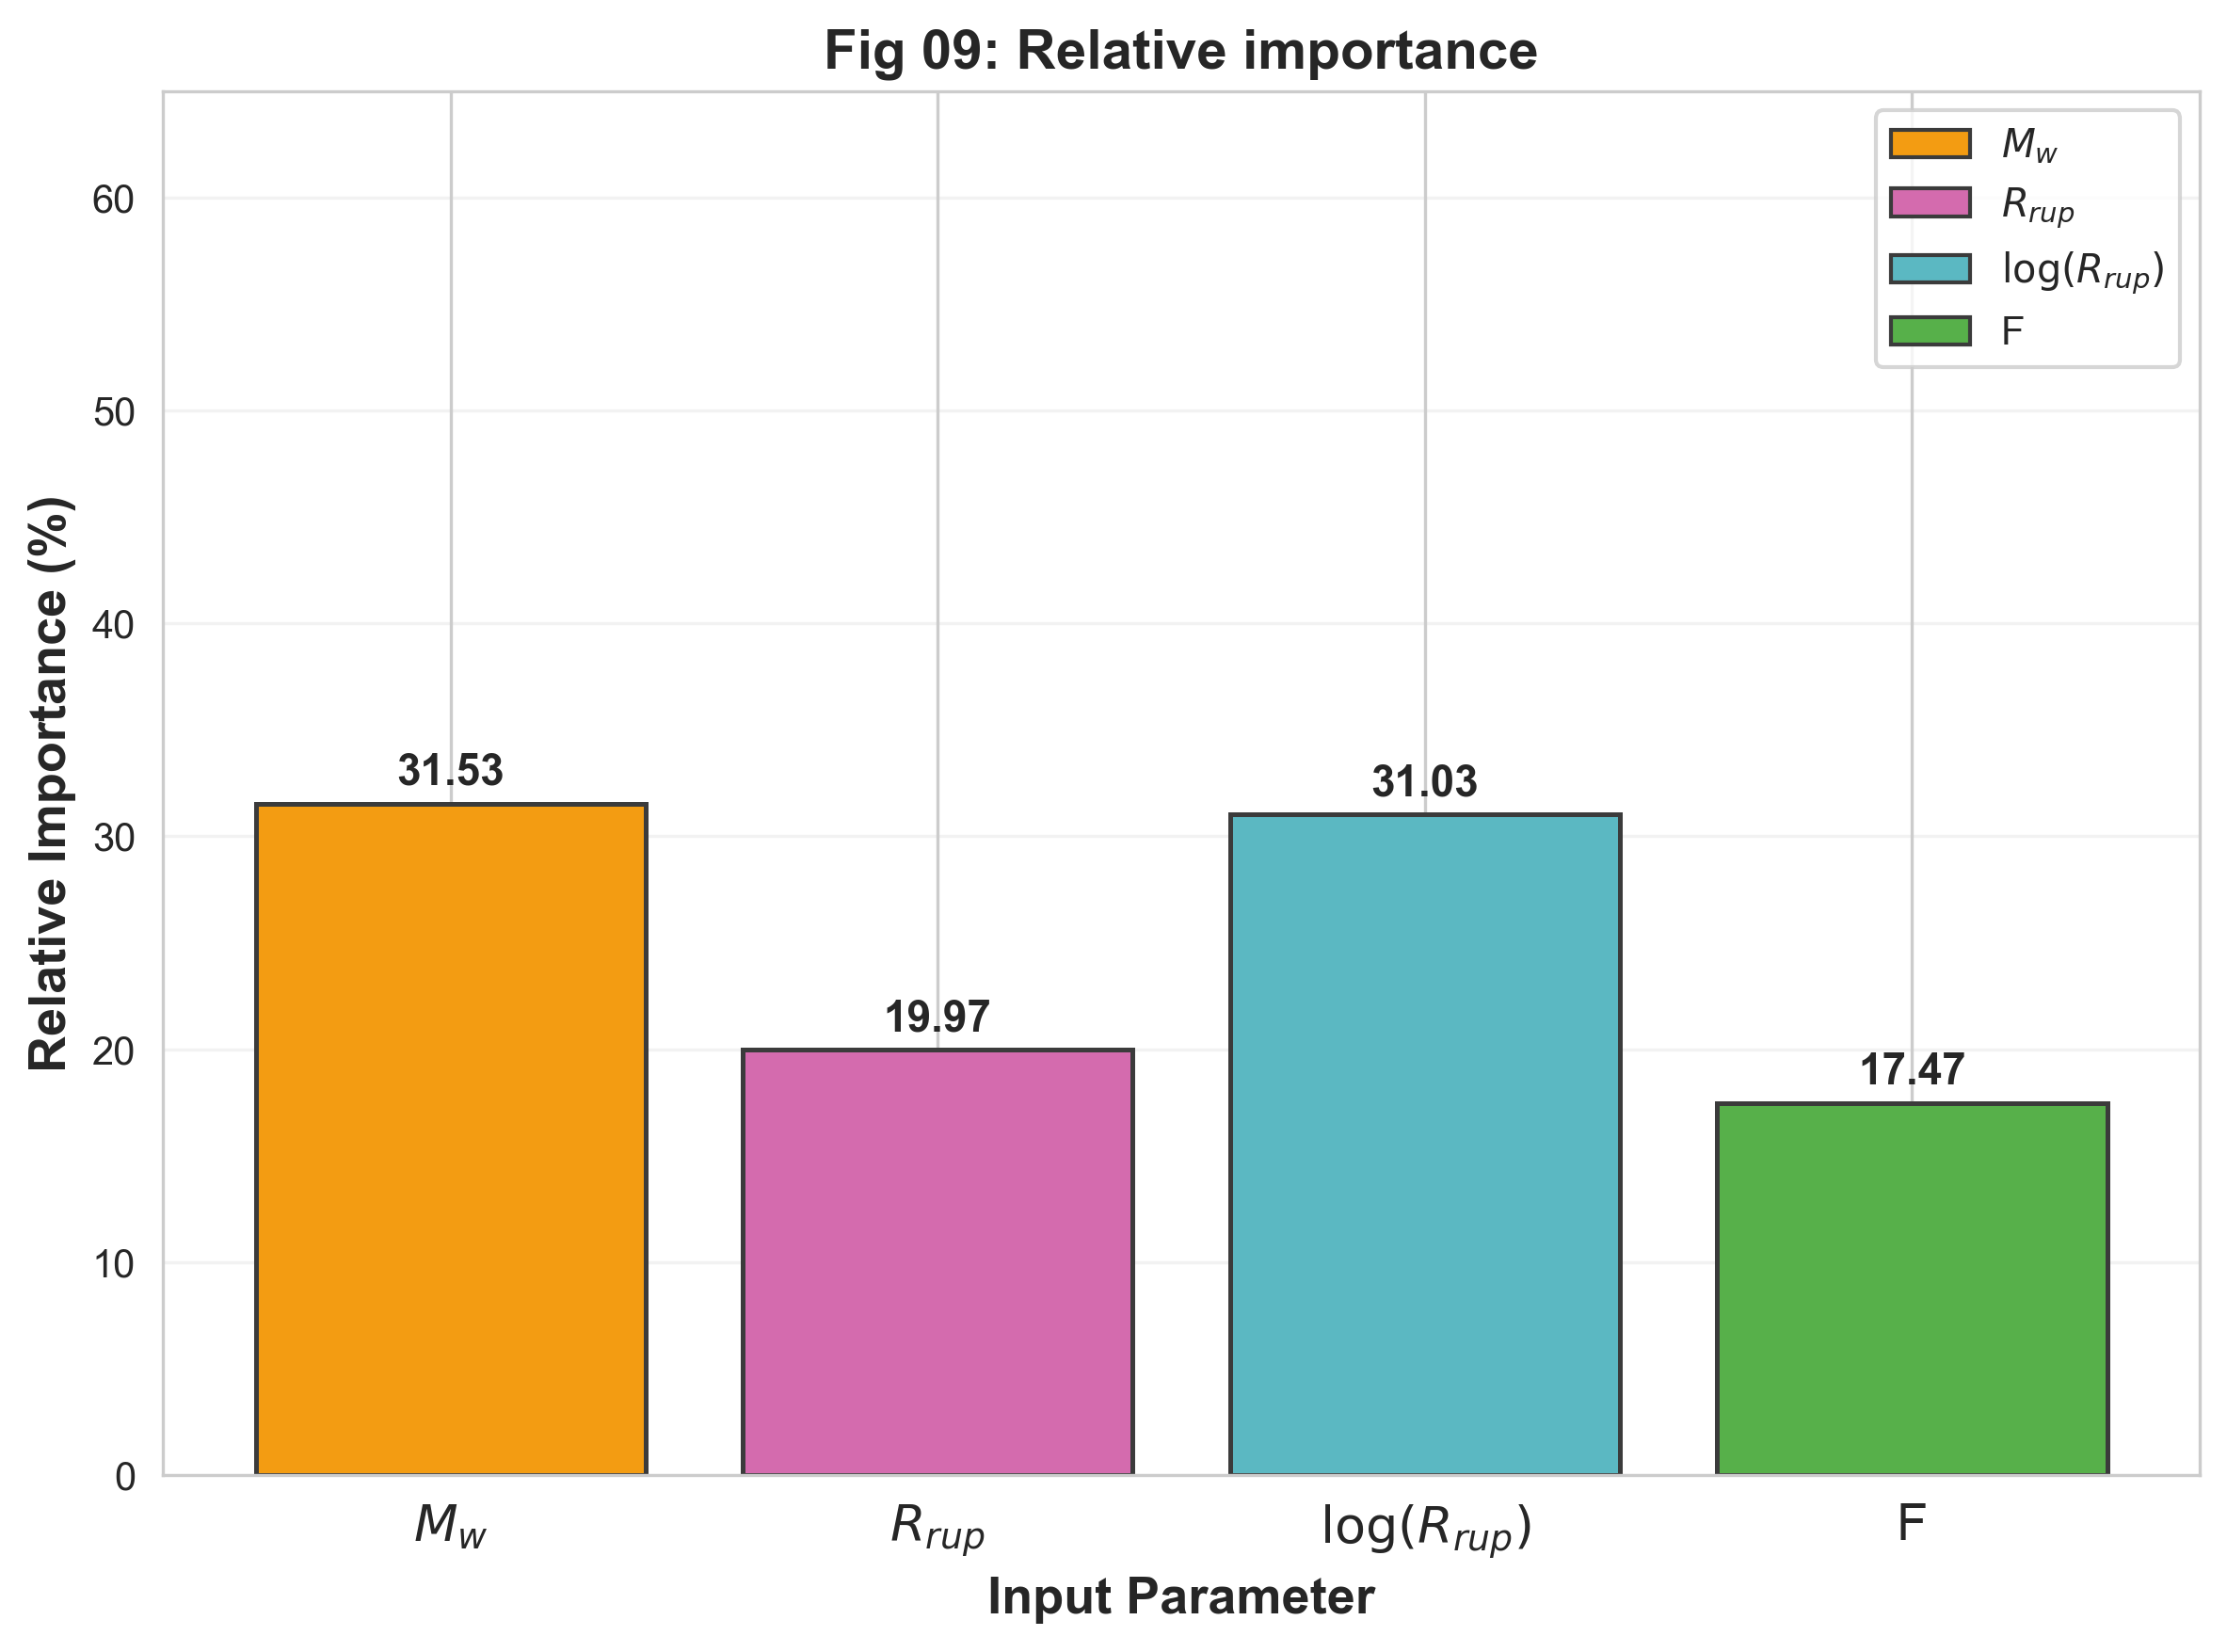
\includegraphics[width=0.7\linewidth]{fig09_feature_importance}
  \caption{Mean absolute SHAP values summed across all 30 IMs, showing
           global feature importance rankings.}
  \label{fig:feature_importance}
\end{figure}

The interaction feature $M_w \cdot \ln R_{jb}$ and log-distance $\ln R_{jb}$
are the two dominant predictors across all spectral periods, consistent with
the standard functional form of empirical GMMs.
$M_w$ and $\ln V_{s30}$ are the next most important features.
$Z_{tor}$ and the finite-fault-model flag contribute more at longer periods,
where rupture geometry has a stronger influence on the spectral shape.
The quadratic term $M_w^2$ provides marginal but consistent improvement,
particularly at intermediate magnitudes.

% ===================================================================
%  7. DISCUSSION
% ===================================================================
\section{Discussion}
\label{sec:discussion}

\subsection{Why BiLSTM for the Spectral Problem?}

The fundamental insight is that the 30 output IMs are not independent: they
are evaluations of the same underlying stochastic process (the transfer function
between source motion and structural response) at different oscillator
frequencies.
Standard multi-output MLPs treat them as independent, which is statistically
suboptimal.
The BiLSTM's hidden state propagates spectral information across period steps,
effectively implementing a learned form of spectral cross-correlation.
This is particularly valuable at periods where data are sparse (long periods
for subduction events are better constrained than in crustal datasets, but
still have higher variance).

The bidirectional processing is physically motivated: spectral behaviour in
the short-period range ($T < 0.1$~s) is controlled by high-frequency radiation
efficiency (related to stress drop and focal mechanism), while long-period
behaviour ($T > 1$~s) is controlled by rupture area and low-$V_{s30}$
amplification.
Processing in both directions allows the LSTM states to simultaneously encode
both regimes.

\subsection{Period Embedding as a Spectral Interpolator}

The continuous period embedding (Section~\ref{sec:period_embed}) makes the
model a spectral interpolator: given a feature vector $\mathbf{x}$, the user
can query the model at \emph{any} period by providing the corresponding
$\ln T$ as input to the Period MLP, without retraining.
This is a significant practical advantage over lookup-table or one-hot period
encodings, which are limited to the discrete periods seen during training.

\subsection{Physical Plausibility and Extrapolation}

All four sensitivity checks (magnitude, distance, $V_{s30}$, $Z_{tor}$) yield
monotonic spectral ordering with zero crossings (Section~\ref{sec:sensitivity}).
This is a strong, non-trivial result: the BiLSTM learned correct physical
ordering without any explicit monotonicity constraint, relying instead on the
inductive bias of the spectral-sequence formulation combined with the Huber
loss and smoothness regulariser.

Extrapolation to conditions outside the training range---e.g., $M_w > 9$,
$R_{jb} > 800$~km---should be approached cautiously, as with any data-driven
model.
At very high magnitudes the BiLSTM may not reproduce finite-fault saturation
effects that dedicated functional forms explicitly encode.

\subsection{Total Sigma and Aleatory Variability}

The total sigma values in Table~\ref{tab:sigma} represent the irreducible
aleatory variability in the prediction: the scatter not explained by the eight
input features.
Our $\sigma_T(\text{PGA}) = 0.625$ compares favourably with published
subduction GMMs, which typically report $\sigma_T \approx 0.65$--$0.80$ for
interface events \citep{Abrahamson2016,Zhao2006,Ghofrani2014}.
The reduction is partly attributable to the flexibility of the ML model
(lower bias than parametric forms) and partly to the inclusion of both
interface and intraslab events, which reduces the dynamic range of source
characteristics that the model must span compared with single-regime GMMs.

It is important to note that we do not report epistemic uncertainty on the
model parameters themselves; this is a limitation of the current work.
Bayesian neural networks or ensembles \citep{Lakshminarayanan2017} could
provide model-uncertainty estimates alongside predictions, which is an
important direction for future work.

\subsection{Comparison to Prior Neural-Network GMMs}

Direct quantitative comparison with published ML GMMs is complicated by
differences in training data, target IMs, and validation methodology.
Qualitatively, the performance levels reported here ($r \ge 0.916$ for all IMs)
are in line with or exceed those reported by \citet{Derras2014} for European
GMMs and \citet{Sahakian2018} for California, while simultaneously predicting
30 IMs in a single forward pass rather than one at a time.
The 16\% reduction in $\sigma_T(\text{PGA})$ relative to BC~Hydro
\citep{Abrahamson2016} is consistent with the general finding that flexible
ML models reduce parametric bias compared with prescribed functional forms.

\subsection{Limitations}

\begin{enumerate}[leftmargin=*,label=\textbf{L\arabic*.}]
  \item \textbf{Subduction-specific training data.}
    The model is trained on NGA-Subduction records and is not expected to
    generalise to crustal or stable continental events.
  \item \textbf{No epistemic uncertainty.}
    Point predictions are provided; model-parameter uncertainty is not quantified.
  \item \textbf{Proxy event/site grouping.}
    Residual decomposition uses magnitude and $V_{s30}$ bins as proxies for
    earthquake events and recording stations; access to event and station IDs
    would enable more rigorous mixed-effects analysis.
  \item \textbf{No basin or directivity terms.}
    Features such as basin depth ($Z_{1.0}$, $Z_{2.5}$) and source directivity
    are not included, limiting applicability in near-fault scenarios.
\end{enumerate}

% ===================================================================
%  8. CONCLUSIONS
% ===================================================================
\section{Conclusions}
\label{sec:conclusion}

We presented BiLSTM-GMM, a bidirectional LSTM ground motion model that
reformulates simultaneous multi-output spectral prediction as a
sequence-to-sequence learning problem.
The key innovations---spectral-sequence formulation, dual-branch architecture
with continuous period embedding, residual feature encoding, and
physics-informed spectral regularisation---result in a model that:
\begin{enumerate}[leftmargin=*]
  \item Predicts PGA, 28 PSA ordinates (0.01--10~s), and PGV simultaneously in
        a single forward pass with test $R^2 = 0.925$.
  \item Achieves per-IM Pearson $r = 0.916$--0.956 across all 30 IMs on the
        held-out test set.
  \item Reproduces physically expected monotonic scaling with magnitude,
        distance, site condition, and rupture depth, as verified by sensitivity
        analysis.
  \item Produces total sigma values ($\sigma_T = 0.524$--$0.739$~ln) competitive
        with or lower than published empirical subduction GMMs.
  \item Provides a generalisation pathway to arbitrary periods through the
        continuous period embedding, without retraining.
\end{enumerate}

The sequence-aware formulation is general: it can be applied to any multi-output
ground motion prediction problem where the outputs are naturally ordered (by
period, frequency, or depth).
Future work includes Bayesian uncertainty quantification, incorporation of basin
and directivity terms, and extension to joint source-path-site physics-informed
architectures.

\section*{Data and Code Availability}

The NGA-Subduction flatfile is publicly available from the PEER Ground Motion
Database.
Model weights, training scripts, and the interactive prediction pipeline
(\texttt{sda\_predict.py}) are available on request from the authors.

\section*{Acknowledgements}

The authors thank the Pacific Earthquake Engineering Research (PEER) Center for
maintaining the NGA-Subduction database.

% ===================================================================
%  REFERENCES
% ===================================================================
\bibliographystyle{plainnat}
\begin{thebibliography}{99}

\bibitem[Abrahamson et~al.(2016)]{Abrahamson2016}
Abrahamson, N.A., Gregor, N., and Addo, K. (2016).
BC Hydro ground motion prediction equations for subduction earthquakes.
\textit{Earthquake Spectra}, 32(1), 23--44.
\doi{10.1193/051712EQS188MR}

\bibitem[Al-Atik et~al.(2010)]{Al-Atik2010}
Al-Atik, L., Abrahamson, N., Bommer, J.J., Scherbaum, F., Cotton, F.,
and Kuehn, N. (2010).
The variability of ground-motion prediction models and its components.
\textit{Seismological Research Letters}, 81(5), 794--801.
\doi{10.1785/gssrl.81.5.794}

\bibitem[Atkinson and Boore(2003)]{Atkinson2003}
Atkinson, G.M. and Boore, D.M. (2003).
Empirical ground-motion relations for subduction-zone earthquakes and their
application to Cascadia and other regions.
\textit{Bulletin of the Seismological Society of America}, 93(4), 1703--1729.
\doi{10.1785/0120020156}

\bibitem[Ba et~al.(2016)]{Ba2016}
Ba, J.L., Kiros, J.R., and Hinton, G.E. (2016).
Layer normalization.
\textit{arXiv preprint} arXiv:1607.06450.

\bibitem[Baker and Cornell(2006)]{Baker2006}
Baker, J.W. and Cornell, C.A. (2006).
Spectral shape, epsilon and record selection.
\textit{Earthquake Engineering \& Structural Dynamics}, 35(9), 1077--1095.
\doi{10.1002/eqe.571}

\bibitem[Baker and Jayaram(2008)]{Baker2008}
Baker, J.W. and Jayaram, N. (2008).
Correlation of spectral acceleration values from NGA ground motion models.
\textit{Earthquake Spectra}, 24(1), 299--317.
\doi{10.1193/1.2857544}

\bibitem[Bakir et~al.(2007)]{Bakir2007}
Bakir, G., Hofmann, T., Sch\"{o}lkopf, B., Smola, A.J., Taskar, B.,
and Vishwanathan, S.V.N. (2007).
\textit{Predicting Structured Data}. MIT Press, Cambridge, MA.

\bibitem[Bayona et~al.(2022)]{Bayona2022}
Bayona, J.A., Savran, W., Strader, A., Marzocchi, W., and Jordan, T.H. (2022).
Prospective evaluation of multiplicative hybrid earthquake forecasting models
in California.
\textit{Geophysical Journal International}, 229(3), 1736--1753.
\doi{10.1093/gji/ggac018}

\bibitem[Boore et~al.(2014)]{Boore2014}
Boore, D.M., Stewart, J.P., Seyhan, E., and Atkinson, G.M. (2014).
NGA-West2 equations for predicting PGA, PGV, and 5\% damped PSA for shallow
crustal earthquakes.
\textit{Earthquake Spectra}, 30(3), 1057--1085.
\doi{10.1193/070113EQS184M}

\bibitem[Bozorgnia et~al.(2014)]{Bozorgnia2014}
Bozorgnia, Y., Abrahamson, N.A., Al-Atik, L., Ancheta, T.D., et~al. (2014).
NGA-West2 research project.
\textit{Earthquake Spectra}, 30(3), 973--987.
\doi{10.1193/072113EQS209M}

\bibitem[Campbell and Bozorgnia(2014)]{Campbell2014}
Campbell, K.W. and Bozorgnia, Y. (2014).
NGA-West2 ground motion model for the average horizontal components of PGA,
PGV, and 5\% damped linear acceleration response spectra.
\textit{Earthquake Spectra}, 30(3), 1087--1115.
\doi{10.1193/062913EQS175M}

\bibitem[Caruana(1997)]{Caruana1997}
Caruana, R. (1997).
Multitask learning.
\textit{Machine Learning}, 28(1), 41--75.
\doi{10.1023/A:1007379606734}

\bibitem[Chiou and Youngs(2014)]{Chiou2014}
Chiou, B.S.-J. and Youngs, R.R. (2014).
Update of the Chiou and Youngs NGA model for the average horizontal component
of peak ground motion and response spectra.
\textit{Earthquake Spectra}, 30(3), 1117--1153.
\doi{10.1193/072813EQS219M}

\bibitem[Cornell(1968)]{Cornell1968}
Cornell, C.A. (1968).
Engineering seismic risk analysis.
\textit{Bulletin of the Seismological Society of America}, 58(5), 1583--1606.

\bibitem[Derras et~al.(2014)]{Derras2014}
Derras, B., Bard, P.Y., and Cotton, F. (2014).
Towards fully data-driven ground-motion prediction models for Europe.
\textit{Bulletin of Earthquake Engineering}, 12(1), 495--516.
\doi{10.1007/s10518-013-9481-0}

\bibitem[Derras et~al.(2016)]{Derras2016}
Derras, B., Bard, P.Y., and Cotton, F. (2016).
Site-condition proxies, ground motion variability, and data-driven GMPEs.
\textit{Earthquake Spectra}, 33(1), 35--60.
\doi{10.1193/060215EQS082M}

\bibitem[Ghofrani and Atkinson(2014)]{Ghofrani2014}
Ghofrani, H. and Atkinson, G.M. (2014).
Ground-motion prediction equations for interface earthquakes of $M6$--9 based
on empirical data from Japan.
\textit{Bulletin of Earthquake Engineering}, 12, 549--571.
\doi{10.1007/s10518-013-9533-5}

\bibitem[Graves(2013)]{Graves2013}
Graves, A., Mohamed, A., and Hinton, G.E. (2013).
Speech recognition with deep recurrent neural networks.
In \textit{IEEE International Conference on Acoustics, Speech and Signal
Processing (ICASSP)}, pp.\ 6645--6649.
\doi{10.1109/ICASSP.2013.6638947}

\bibitem[He et~al.(2016)]{He2016}
He, K., Zhang, X., Ren, S., and Sun, J. (2016).
Deep residual learning for image recognition.
In \textit{Proc.\ IEEE Conference on Computer Vision and Pattern Recognition
(CVPR)}, pp.\ 770--778.
\doi{10.1109/CVPR.2016.90}

\bibitem[Hendrycks and Gimpel(2016)]{Hendrycks2016}
Hendrycks, D. and Gimpel, K. (2016).
Gaussian error linear units (GELUs).
\textit{arXiv preprint} arXiv:1606.08415.

\bibitem[Hochreiter and Schmidhuber(1997)]{Hochreiter1997}
Hochreiter, S. and Schmidhuber, J. (1997).
Long short-term memory.
\textit{Neural Computation}, 9(8), 1735--1780.
\doi{10.1162/neco.1997.9.8.1735}

\bibitem[Huber(1964)]{Huber1964}
Huber, P.J. (1964).
Robust estimation of a location parameter.
\textit{The Annals of Mathematical Statistics}, 35(1), 73--101.
\doi{10.1214/aoms/1177703732}

\bibitem[Jayaram and Baker(2009)]{Jayaram2009}
Jayaram, N. and Baker, J.W. (2009).
Correlation model for spatially distributed ground-motion intensities.
\textit{Earthquake Engineering \& Structural Dynamics}, 38(15), 1687--1708.
\doi{10.1002/eqe.922}

\bibitem[Khosravikia and Clayton(2021)]{Khosravikia2021}
Khosravikia, F. and Clayton, P. (2021).
Updated ANN-based ground motion model for Texas, Oklahoma, and Kansas.
\textit{Earthquake Engineering \& Structural Dynamics}, 50(2), 441--462.
\doi{10.1002/eqe.3341}

\bibitem[Kuehn and Scherbaum(2015)]{Kuehn2015}
Kuehn, N.M. and Scherbaum, F. (2015).
Ground-motion prediction model building: a multilevel approach.
\textit{Bulletin of Earthquake Engineering}, 13, 2481--2491.
\doi{10.1007/s10518-015-9732-3}

\bibitem[Lakshminarayanan et~al.(2017)]{Lakshminarayanan2017}
Lakshminarayanan, B., Pritzel, A., and Blundell, C. (2017).
Simple and scalable predictive uncertainty estimation using deep ensembles.
In \textit{Advances in Neural Information Processing Systems (NeurIPS)}, 30.

\bibitem[Loshchilov and Hutter(2019)]{Loshchilov2019}
Loshchilov, I. and Hutter, F. (2019).
Decoupled weight decay regularization.
In \textit{International Conference on Learning Representations (ICLR 2019)}.

\bibitem[Lundberg and Lee(2017)]{Lundberg2017}
Lundberg, S.M. and Lee, S.-I. (2017).
A unified approach to interpreting model predictions.
In \textit{Advances in Neural Information Processing Systems (NeurIPS)}, 30.
\doi{10.48550/arXiv.1705.07874}

\bibitem[McGuire(2004)]{McGuire2004}
McGuire, R.K. (2004).
\textit{Seismic Hazard and Risk Analysis}.
Earthquake Engineering Research Institute, Oakland, CA.

\bibitem[Perol et~al.(2018)]{Perol2018}
Perol, T., Gharbi, M., and Denolle, M. (2018).
Convolutional neural network for earthquake detection and location.
\textit{Science Advances}, 4(2), e1700578.
\doi{10.1126/sciadv.1700578}

\bibitem[Sahakian et~al.(2018)]{Sahakian2018}
Sahakian, V., Baltay, A., Hanks, T., Boore, D., and Abrahamson, N. (2018).
Decomposing leftovers: event, path, and site residuals for a small-magnitude
ground motion model.
\textit{Bulletin of the Seismological Society of America}, 108(5A), 2478--2492.
\doi{10.1785/0120170376}

\bibitem[Schuster et~al.(1997)]{Schuster1997}
Schuster, M. and Paliwal, K.K. (1997).
Bidirectional recurrent neural networks.
\textit{IEEE Transactions on Signal Processing}, 45(11), 2673--2681.
\doi{10.1109/78.650093}

\bibitem[Smith(2019)]{Smith2019}
Smith, L.N. and Topin, N. (2019).
Super-convergence: very fast training of neural networks using large
learning rates.
In \textit{Artificial Intelligence and Machine Learning for Multi-Domain
Operations Applications}, Proc.\ SPIE, 11006.
\doi{10.1117/12.2520589}

\bibitem[Zhao et~al.(2006)]{Zhao2006}
Zhao, J.X., Zhang, J., Asano, A., Ohno, Y., et~al. (2006).
Attenuation relations of strong ground motion in Japan using site
classification based on predominant period.
\textit{Bulletin of the Seismological Society of America}, 96(3), 898--913.
\doi{10.1785/0120050122}

\end{thebibliography}

\end{document}
